\documentclass[11pt]{article}

\usepackage[margin=1.2in]{geometry}
\usepackage{amsmath,amssymb}
\usepackage[T1]{fontenc}
\usepackage[utf8]{inputenc}
\usepackage{lmodern}
\usepackage{microtype}
\usepackage{booktabs}
\usepackage[hidelinks,hypertexnames=false]{hyperref}
\usepackage{parskip}
\usepackage{enumitem}
\PassOptionsToPackage{dvipsnames}{xcolor}
\usepackage{tikz}
\usepackage{xcolor}
\usetikzlibrary{positioning, shapes.geometric, decorations.pathmorphing, decorations.pathreplacing, arrows.meta, calc, patterns}
\usepackage{float}
\usepackage{tcolorbox}
\newtcolorbox{keymessage}{%
  colback=blue!3, colframe=blue!40!black,
  fonttitle=\bfseries\small, title=Key Message,
  boxrule=0.5pt, arc=2pt, left=6pt, right=6pt, top=4pt, bottom=4pt
}

\title{The Map and the Territory:\\
A Constructive History of Mathematical Physics\\[6pt]
\large Version 1.1 (02/09/2026)}
\author{Paul Chun-Kit Lee\\[2pt]
\small New York University}
\date{February 2026}

\begin{document}
\maketitle

\begin{abstract}
This essay tells the story of 150~years of mathematical physics from an unfamiliar angle.
A machine-verified research programme---approximately 12,000~lines of formally checked proofs in the Lean~4 proof assistant---has established that every empirical prediction of quantum and statistical mechanics examined so far can be derived using only the most elementary constructive logic, without the law of excluded middle or any principle of omniscience.
The elaborate classical superstructure of modern physics---infinite-dimensional Hilbert spaces, thermodynamic limits, path integrals, singularity theorems---enters only through idealizations that no finite laboratory can instantiate.
This essay traces how classical logic was progressively imported into mathematical physics from the 1870s onward, what it cost at each stage, what constructive alternatives existed or could have been used instead, and what the pattern implies for the current state of theoretical physics.
This is Paper~12 in the Constructive Calibration Programme, a companion to the formal synthesis (Paper~10) \cite{Lee2026paper10}, written for a broader audience.
The calibration covers quantum states, static structures, exactly solvable models, decoherence bounds, conservation laws, and Born-rule probabilities; time evolution, scattering amplitudes, and real-time path integrals remain uncalibrated.
\end{abstract}

% ============================================================
\section{The Cellar and the Cathedral}
% ============================================================

The most precise prediction in the history of science is a number: the anomalous magnetic moment of the electron, usually called $g{-}2$.
Quantum electrodynamics predicts this quantity to roughly twelve decimal places, and experiment confirms it.
The agreement is so exact that if you measured the distance from New York to Los Angeles to the same relative precision, you would be accurate to the width of a human hair.

Here is the quiet scandal behind that triumph.
Every step of the actual computation is finite arithmetic.
A physicist draws a Feynman diagram---a small picture of particles interacting---and translates it into a definite integral over a finite number of momentum variables.
She evaluates the integral numerically, adds contributions from a finite number of diagrams at each level of approximation, and arrives at a rational number with controlled error bars.
Every operation could be performed by a mechanical calculator given enough time.
There is no step that requires surveying an infinite set, deciding an undecidable question, or asserting the existence of a completed infinite object.

And yet the formalism in which this computation is embedded is a cathedral of infinities.
The path integral---the foundational tool of quantum field theory---is, in its continuum formulation, an ``integral'' over an infinite-dimensional space of field configurations for which no mathematically rigorous measure exists in general.
(Euclidean lattice path integrals---Wilson's 1974 construction \cite{Wilson1974}---are mathematically rigorous but operate on finite lattices, i.e., at BISH.)
Fock space, the mathematical arena for multi-particle quantum mechanics, is an infinite-dimensional tensor product.
Renormalization, the procedure that extracts finite predictions from divergent expressions, involves manipulations with quantities that are formally infinite.
The vacuum state---the ``empty'' starting point of every calculation---is a vector in an infinite-dimensional space whose properties encode the entire structure of the theory.

\begin{figure}[ht]
\centering
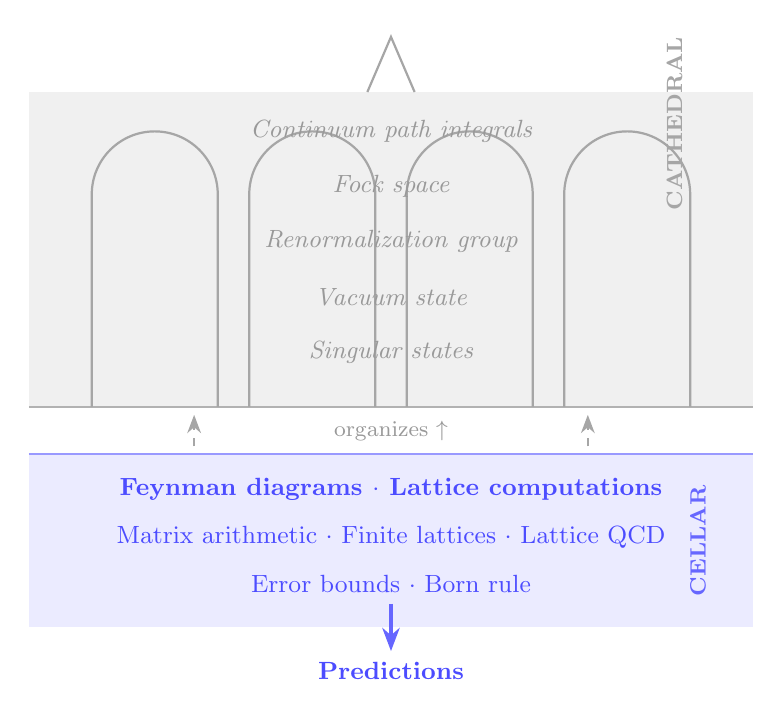
\begin{tikzpicture}[
  >=Stealth,
  every node/.style={font=\small}
]
% Cathedral (upper level) — shaded gray
\fill[gray!12] (-4.6, 2.8) rectangle (4.6, 6.8);
\draw[thick, gray!60] (-4.6, 2.8) -- (4.6, 2.8);
% Arches
\foreach \x in {-3, -1, 1, 3} {
  \draw[gray!70, thick] (\x-0.8, 2.8) -- (\x-0.8, 5.5) arc (180:0:0.8) -- (\x+0.8, 2.8);
}
% Spire
\draw[gray!70, thick] (-0.3, 6.8) -- (0, 7.5) -- (0.3, 6.8);
% Cathedral labels
\node[font=\small\itshape, gray!80] at (0, 6.3) {Continuum path integrals};
\node[font=\small\itshape, gray!80] at (0, 5.6) {Fock space};
\node[font=\small\itshape, gray!80] at (0, 4.9) {Renormalization group};
\node[font=\small\itshape, gray!80] at (0, 4.2) {Vacuum state};
\node[font=\small\itshape, gray!80] at (0, 3.5) {Singular states};
\node[font=\footnotesize\bfseries, gray!70] at (3.6, 6.4) {\rotatebox{90}{CATHEDRAL}};

% Cellar (lower level) — shaded blue
\fill[blue!8] (-4.6, 0) rectangle (4.6, 2.2);
\draw[thick, blue!40] (-4.6, 2.2) -- (4.6, 2.2);
% Cellar labels
\node[font=\small\bfseries, blue!70] at (0, 1.75) {Feynman diagrams $\cdot$ Lattice computations};
\node[font=\small, blue!70] at (0, 1.15) {Matrix arithmetic $\cdot$ Finite lattices $\cdot$ Lattice QCD};
\node[font=\small, blue!70] at (0, 0.55) {Error bounds $\cdot$ Born rule};
\node[font=\footnotesize\bfseries, blue!60] at (3.9, 1.1) {\rotatebox{90}{CELLAR}};

% Arrow: predictions flow up
\draw[->, very thick, blue!60] (0, 0.3) -- (0, -0.3) node[below, font=\small\bfseries, blue!70] {Predictions};

% Arrow: formalism sits above
\draw[->, thick, gray!70, dashed] (-2.5, 2.3) -- (-2.5, 2.7);
\draw[->, thick, gray!70, dashed] (2.5, 2.3) -- (2.5, 2.7);
\node[font=\footnotesize, gray!80] at (0, 2.5) {organizes $\uparrow$};

\end{tikzpicture}
\caption{The cellar and the cathedral. Every empirical prediction of quantum field theory (below) is a finite computation---BISH. The infinite-dimensional formalism (above) organizes the computations but is not itself physically instantiated.}
\label{fig:cellar-cathedral}
\end{figure}

The predictions come from the cellar.
The cathedral sits above: beautiful, architecturally magnificent, and largely empty.
Almost nobody computes a continuum path integral; in perturbative QFT, they compute Feynman diagrams, and in lattice QCD, they evaluate discretized path integrals on finite lattices---both BISH operations.
Nobody works in Fock space; they work with definite, finite numbers of particles.
The infinite-dimensional superstructure is a mnemonic---a way of organizing the finite computations---but the physics, the part that touches experiment, lives in the finite arithmetic below (Figure~\ref{fig:cellar-cathedral}).

This essay is about the gap between the cellar and the cathedral.
It is about the question: how much of the mathematical apparatus of physics describes the physical world, and how much describes the mathematician's toolkit?
For the first time, a machine-verified research programme can answer this question with mathematical precision.
The answer is surprising, and it reaches back 150~years.
Every empirical prediction we have examined---across quantum mechanics, statistical mechanics, and general relativity---lives at the most elementary level of constructive logic.
The classical superstructure, with its completed infinities and its implicit appeals to omniscience over infinite sets, is the mapmaker's convention.
Nature, it appears, speaks a simpler language.

A word of framing before we proceed.
The map is not useless---it is an extraordinarily effective organizing tool.
Classical mathematics has powered the greatest quantitative achievements in the history of science.
But the map is not the territory.
The thesis of this essay is not that the classical formalism is wrong, but that it contains more structure than the physics requires, and that the excess structure has gradually been mistaken for reality.
The constructive hierarchy provides a precise tool for separating the territory from the mapmaker's conventions.

\begin{keymessage}
Every empirical prediction of QFT examined in this programme is finite arithmetic --- constructive analysis at BISH.
The infinite-dimensional formalism organizes computations but is not physically instantiated.
The predictions come from the cellar; the cathedral is the mathematician's convenience.
\end{keymessage}

A scope note: the calibration programme examines quantum states, static structures, and specific exactly solvable models---not quantum dynamics.
Time evolution, scattering amplitudes, the S-matrix, and real-time path integrals remain uncalibrated.
``BISH'' throughout this essay means Bishop-style constructive analysis---which includes real-valued computation with explicit moduli of convergence, not merely discrete or finite arithmetic.
The claims about empirical predictions should be read with both limitations in mind.


% ============================================================
\section{What Physicists Don't Know They're Assuming}
% ============================================================

To understand what the research programme has discovered, you need to understand a distinction that most physicists have never encountered: the difference between levels of \emph{logical strength} in mathematics.

Before describing the hierarchy, a crucial clarification.
The hierarchy of logical strength (BISH $<$ WLPO $<$ LPO $<$ LEM) measures what \emph{principles} a proof requires---what kind of assertions about infinite sets you must accept.
This is entirely different from Turing undecidability, which measures what no \emph{algorithm} can compute regardless of the axioms you accept.
A problem can be Turing-decidable yet require LPO to prove (the thermodynamic limit), or Turing-undecidable yet live outside the omniscience hierarchy entirely (the spectral gap problem of Cubitt et~al.\ \cite{Cubitt2015}, which is Turing-undecidable).
The spectral gap is undecidable in the sense that no algorithm can determine the answer from a Hamiltonian's local rules; this is not ``a level above LEM'' in the logical hierarchy but an orthogonal phenomenon.
Throughout this essay, ``logical strength'' refers to the constructive hierarchy, not to computability in the Turing sense.

Consider an infinite hotel with rooms numbered 1, 2, 3, and so on.
You want to know whether every room is empty.
Here are four different things you might be allowed to assert, each representing a different level of logical power.

At the first level---call it \textbf{BISH}, for Bishop-style constructive mathematics \cite{Bishop1967}---you can check rooms one by one, and you can report what you find.
If you have a proof that works for every room (a master key, say, that shows no guest could possibly be registered), you may declare ``all empty.''
If you find an occupied room, you may point to it and say ``room 47 is occupied.''
But you may \emph{not} declare ``they're all empty'' without a universal proof, and you may not declare ``someone's home'' without producing the room number.
You claim only what you can demonstrate.

At the second level---\textbf{WLPO}, the Weak Limited Principle of Omniscience---you gain a modest superpower.
You may assert either ``all rooms are empty'' \emph{or} ``it is not the case that all rooms are empty.''
But in the second case, you do not need to produce the occupied room.
You know something is there; you just cannot point to it.

At the third level---\textbf{LPO}, the Limited Principle of Omniscience---you have full dichotomy.
Either ``all rooms are empty'' or ``here is the occupied room.''\footnote{Formally: for any binary sequence $\alpha : \mathbb{N} \to \{0,1\}$, either $\alpha(n) = 0$ for all $n$, or there exists $n$ with $\alpha(n) = 1$.}
No ambiguity, no gap between knowing something exists and finding it.

At the fourth level---\textbf{LEM}, the Law of Excluded Middle, which is the logic of standard mathematics---you can answer \emph{any} yes-or-no question about the hotel instantly.
Not just occupancy: any question whatsoever, about any collection of mathematical objects, has a definite true-or-false answer, whether or not you can determine which.

These levels form a strict hierarchy: BISH is the weakest, LEM is the strongest, and each level implies all those below it but not vice versa \cite{BridgesVita2006, BridgesRichman1987}.
The separations are strict---there are mathematical universes where WLPO holds but LPO fails, and universes where LPO holds but LEM fails.

The hierarchy is not esoteric.
Each step up the ladder is a specific claim about your ability to decide questions involving infinite collections.
BISH says: decide only what you can verify by a finite procedure.
WLPO says: you may know that something is true ``in principle'' without exhibiting a witness.
LPO says: you may decide existence claims about infinite sequences.
LEM says: everything is decidable, period.

\begin{figure}[ht]
\centering
\resizebox{\textwidth}{!}{%
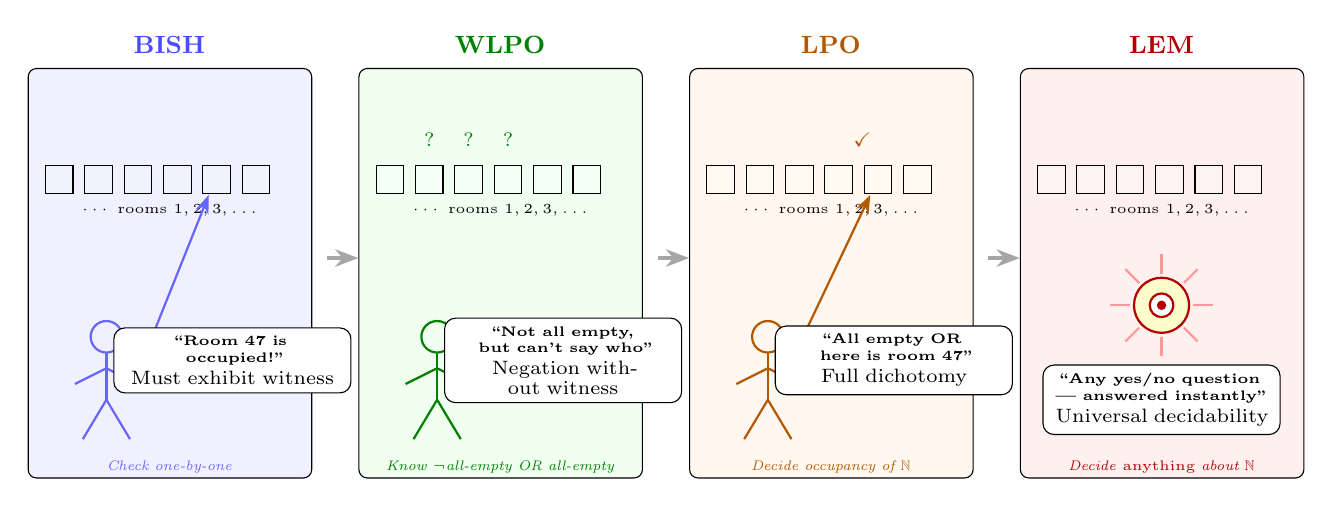
\begin{tikzpicture}[
  >=Stealth,
  panel/.style={draw, rounded corners=3pt, minimum width=3.6cm, minimum height=5.2cm, anchor=south west},
  roomstyle/.style={draw, minimum width=0.35cm, minimum height=0.35cm, inner sep=0pt},
  bubble/.style={draw, rounded corners=4pt, fill=white, font=\tiny, text width=2.8cm, align=center, inner sep=3pt}
]
% Panel 1: BISH
\node[panel, fill=blue!6] (p1) at (0,0) {};
\node[font=\small\bfseries, blue!70] at (1.8, 5.5) {BISH};
% Hotel rooms
\foreach \i in {0,...,5} {
  \node[roomstyle, fill=blue!5] at (0.4+\i*0.5, 3.8) {};
}
\node[font=\tiny] at (1.8, 3.4) {$\cdots$ rooms $1, 2, 3, \ldots$};
% Stick figure checking rooms
\draw[thick, blue!60] (1.0, 1.8) circle (0.2);
\draw[thick, blue!60] (1.0, 1.6) -- (1.0, 1.0);
\draw[thick, blue!60] (1.0, 1.4) -- (0.6, 1.2);
\draw[thick, blue!60] (1.0, 1.4) -- (1.4, 1.2);
\draw[thick, blue!60] (1.0, 1.0) -- (0.7, 0.5);
\draw[thick, blue!60] (1.0, 1.0) -- (1.3, 0.5);
% Arrow pointing to room
\draw[->, thick, blue!60] (1.5, 1.6) -- (2.3, 3.6);
% Speech bubble
\node[bubble] at (2.6, 1.5) {\textbf{``Room 47 is\\occupied!''}\\[2pt]\scriptsize Must exhibit witness};
\node[font=\tiny\itshape, blue!60] at (1.8, 0.15) {Check one-by-one};

% Panel 2: WLPO
\node[panel, fill=green!6] (p2) at (4.2,0) {};
\node[font=\small\bfseries, green!50!black] at (6.0, 5.5) {WLPO};
\foreach \i in {0,...,5} {
  \node[roomstyle, fill=green!5] at (4.6+\i*0.5, 3.8) {};
}
\node[font=\tiny] at (6.0, 3.4) {$\cdots$ rooms $1, 2, 3, \ldots$};
% Stick figure at desk
\draw[thick, green!50!black] (5.2, 1.8) circle (0.2);
\draw[thick, green!50!black] (5.2, 1.6) -- (5.2, 1.0);
\draw[thick, green!50!black] (5.2, 1.4) -- (4.8, 1.2);
\draw[thick, green!50!black] (5.2, 1.4) -- (5.6, 1.2);
\draw[thick, green!50!black] (5.2, 1.0) -- (4.9, 0.5);
\draw[thick, green!50!black] (5.2, 1.0) -- (5.5, 0.5);
% Question marks over rooms
\node[font=\scriptsize, green!50!black] at (5.1, 4.3) {?};
\node[font=\scriptsize, green!50!black] at (5.6, 4.3) {?};
\node[font=\scriptsize, green!50!black] at (6.1, 4.3) {?};
% Speech bubble
\node[bubble] at (6.8, 1.5) {\textbf{``Not all empty,\\but can't say who''}\\[2pt]\scriptsize Negation without witness};
\node[font=\tiny\itshape, green!50!black] at (6.0, 0.15) {Know $\lnot$all-empty OR all-empty};

% Panel 3: LPO
\node[panel, fill=orange!6] (p3) at (8.4,0) {};
\node[font=\small\bfseries, orange!70!black] at (10.2, 5.5) {LPO};
\foreach \i in {0,...,5} {
  \node[roomstyle, fill=orange!5] at (8.8+\i*0.5, 3.8) {};
}
\node[font=\tiny] at (10.2, 3.4) {$\cdots$ rooms $1, 2, 3, \ldots$};
% Oracle figure
\draw[thick, orange!70!black] (9.4, 1.8) circle (0.2);
\draw[thick, orange!70!black] (9.4, 1.6) -- (9.4, 1.0);
\draw[thick, orange!70!black] (9.4, 1.4) -- (9.0, 1.2);
\draw[thick, orange!70!black] (9.4, 1.4) -- (9.8, 1.2);
\draw[thick, orange!70!black] (9.4, 1.0) -- (9.1, 0.5);
\draw[thick, orange!70!black] (9.4, 1.0) -- (9.7, 0.5);
% Check mark and arrow
\draw[->, thick, orange!70!black] (9.8, 1.7) -- (10.7, 3.6);
\node[font=\scriptsize, orange!70!black] at (10.6, 4.3) {\checkmark};
% Speech bubble
\node[bubble] at (11.0, 1.5) {\textbf{``All empty OR\\here is room 47''}\\[2pt]\scriptsize Full dichotomy};
\node[font=\tiny\itshape, orange!70!black] at (10.2, 0.15) {Decide occupancy of $\mathbb{N}$};

% Panel 4: LEM
\node[panel, fill=red!6] (p4) at (12.6,0) {};
\node[font=\small\bfseries, red!70!black] at (14.4, 5.5) {LEM};
\foreach \i in {0,...,5} {
  \node[roomstyle, fill=red!5] at (13.0+\i*0.5, 3.8) {};
}
\node[font=\tiny] at (14.4, 3.4) {$\cdots$ rooms $1, 2, 3, \ldots$};
% God's eye
\draw[thick, red!70!black, fill=yellow!20] (14.4, 2.2) circle (0.35);
\draw[thick, red!70!black, fill=white] (14.4, 2.2) circle (0.15);
\fill[red!70!black] (14.4, 2.2) circle (0.06);
% Rays
\foreach \a in {0,45,...,315} {
  \draw[red!40, thick] (14.4, 2.2) ++ (\a:0.4) -- ++ (\a:0.25);
}
% Speech bubble
\node[bubble] at (14.4, 1.0) {\textbf{``Any yes/no question\\--- answered instantly''}\\[2pt]\scriptsize Universal decidability};
\node[font=\tiny\itshape, red!70!black] at (14.4, 0.15) {Decide \emph{anything} about $\mathbb{N}$};

% Arrows showing hierarchy
\draw[->, very thick, gray!70] (3.8, 2.8) -- (4.2, 2.8);
\draw[->, very thick, gray!70] (8.0, 2.8) -- (8.4, 2.8);
\draw[->, very thick, gray!70] (12.2, 2.8) -- (12.6, 2.8);

\end{tikzpicture}%
}% end resizebox
\caption{The infinite hotel at four logical levels.
\textbf{BISH}: you may assert only what you can verify by finite procedure.
\textbf{WLPO}: you may assert ``not all empty'' without producing the occupied room.
\textbf{LPO}: full dichotomy on infinite sequences---either all empty or exhibit a witness.
\textbf{LEM}: every yes/no question about any mathematical object has a definite answer.
Each level implies all those to its left; the implications are strict.}
\label{fig:hotel}
\end{figure}

Physicists work at the top of this ladder without a second thought.
Every proof in a standard textbook uses the law of excluded middle freely: a particle is either in this region or it isn't; a sequence either converges or it doesn't; a geodesic either terminates or it extends forever.
The question this essay addresses is whether the physics \emph{needs} all that logical power, or whether the predictions would survive with less.

Think of it this way.
Every theorem in a physics textbook has an invisible footnote reading: ``This proof also assumes that you can survey infinite sets in a single glance.''
The research programme described here identifies which theorems genuinely need that footnote and which would stand without it.

\begin{figure}[ht]
\centering
\resizebox{\textwidth}{!}{%
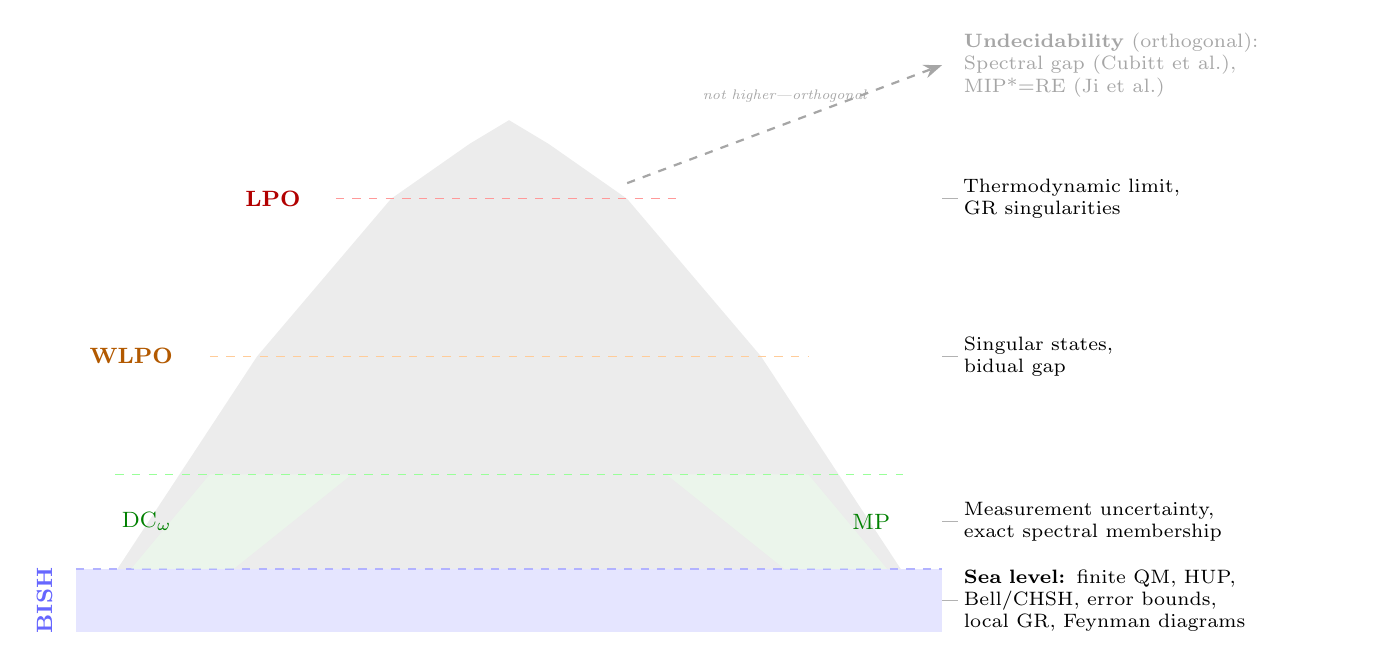
\begin{tikzpicture}[
  >=Stealth,
  every node/.style={font=\small},
  physlabel/.style={font=\scriptsize, text width=4.5cm, align=left, inner sep=2pt}
]
% Mountain body — summit at LPO (y=6.5)
\fill[gray!15] (-5.5,0) -- (-3.2, 3.5) -- (-1.5, 5.5) -- (-0.5, 6.2) -- (0, 6.5) -- (0.5, 6.2) -- (1.5, 5.5) -- (3.2, 3.5) -- (5.5, 0) -- cycle;
% Altitude bands — shaded
\fill[blue!10] (-5.5, 0) -- (-5.5, 0.8) -- (5.5, 0.8) -- (5.5, 0) -- cycle;
\draw[blue!30, dashed] (-5.5, 0.8) -- (5.5, 0.8);
% Sea level label
\node[font=\footnotesize\bfseries, blue!60] at (-5.9, 0.4) {\rotatebox{90}{BISH}};
% Foothills
\fill[green!8, opacity=0.5] (-4.8, 0.8) -- (-3.8, 2.0) -- (-2.0, 2.0) -- (-3.5, 0.8) -- cycle;
\fill[green!8, opacity=0.5] (3.5, 0.8) -- (2.0, 2.0) -- (3.8, 2.0) -- (4.8, 0.8) -- cycle;
\draw[green!40, dashed] (-5.0, 2.0) -- (5.0, 2.0);
\node[font=\footnotesize, green!50!black] at (-4.6, 1.4) {\footnotesize DC$_\omega$};
\node[font=\footnotesize, green!50!black] at (4.6, 1.4) {\footnotesize MP};
% Mountainside
\draw[orange!40, dashed] (-3.8, 3.5) -- (3.8, 3.5);
\node[font=\footnotesize\bfseries, orange!70!black] at (-4.8, 3.5) {WLPO};
% Summit
\draw[red!40, dashed] (-2.2, 5.5) -- (2.2, 5.5);
\node[font=\footnotesize\bfseries, red!70!black] at (-3.0, 5.5) {LPO};

% Undecidability — orthogonal side annotation (arrow points right, not up)
\draw[->, gray!70, dashed, thick] (1.5, 5.7) -- (5.5, 7.2);
\node[font=\scriptsize, gray!70, text width=4.8cm, align=left, inner sep=2pt,
      anchor=west] at (5.7, 7.2)
  {\textbf{Undecidability} (orthogonal):\\Spectral gap (Cubitt et al.),\\MIP*=RE (Ji et al.)};
\node[font=\tiny\itshape, gray!70] at (3.5, 6.8) {not higher---orthogonal};

% Physics labels on right
\node[physlabel, anchor=west] at (5.7, 0.4)
  {\textbf{Sea level:} finite QM, HUP,\\Bell/CHSH, error bounds,\\local GR, Feynman diagrams};
\node[physlabel, anchor=west] at (5.7, 1.4)
  {Measurement uncertainty,\\exact spectral membership};
\node[physlabel, anchor=west] at (5.7, 3.5)
  {Singular states,\\bidual gap};
\node[physlabel, anchor=west] at (5.7, 5.5)
  {Thermodynamic limit,\\GR singularities};

% Connecting lines
\foreach \y/\xr in {0.4/5.5, 1.4/5.5, 3.5/5.5, 5.5/5.5} {
  \draw[gray!60, thin] (5.5, \y) -- (\xr+0.2, \y);
}

\end{tikzpicture}%
}% end resizebox
\caption{The logical geography of mathematical physics, depicted as a mountain.
Sea level (BISH) contains all empirical predictions. Higher altitudes correspond to
greater logical strength---stronger principles, not greater computational complexity.
DC$_\omega$ and MP occupy independent foothills---neither implies the other, and neither
implies WLPO. The summit (LPO) contains the thermodynamic limit and singularity theorems.
Turing undecidability (spectral gap, MIP*=RE) is orthogonal to the logical-strength
hierarchy and is shown as a separate axis rather than a higher altitude.}
\label{fig:mountain}
\end{figure}

To give the hierarchy a visual anchor, imagine a mountain (Figure~\ref{fig:mountain}).
Sea level is BISH---constructive mathematics, finite procedures, the logic of computation.
The foothills are occupied by Dependent Choice and Markov's Principle---modest extensions that allow countable sequences of choices or conclude existence from the impossibility of non-existence.
These two foothills are \emph{independent}: neither implies the other, and neither implies WLPO.
The mountain has ridges running in different directions.
The mountainside is WLPO---where infinite-dimensional analysis begins to part company with finite approximation.
The summit is LPO---the regime of completed infinite limits, thermodynamic idealization, and the convergence of bounded monotone sequences.
The spectral gap problem \cite{Cubitt2015} lies not above the summit but orthogonal to it: Turing undecidability is a constraint on algorithms, not a position in the omniscience hierarchy.

The research programme maps the major theorems of mathematical physics onto this mountain.
The results are striking.
Everything a laboratory does---every preparation, every measurement, every finite computation---lives at sea level.
The idealizations begin on the mountainside, and the summit is populated exclusively by objects that no experiment can instantiate.

\begin{keymessage}
Mathematical physics uses four levels of logical strength: BISH $<$ WLPO $<$ LPO $<$ LEM\@.
Every laboratory operation lives at sea level (BISH).
The question this essay addresses is whether the physics needs the higher altitudes.
\end{keymessage}

% ============================================================
\section{Act~I: The Weierstrass Inheritance (1870--1900)}
% ============================================================

The story begins not with physics but with mathematics.

Before Weierstrass, mathematicians computed with infinitesimals---entities that were simultaneously zero and not zero, useful for deriving results but philosophically disreputable.
In the 1860s and 1870s, Weierstrass and his contemporaries replaced infinitesimals with the epsilon-delta formalism: a limit is not a process of ``approaching'' but a statement about the existence of real numbers satisfying certain inequalities.
This was a triumph of rigor.
It eliminated hand-waving, made proofs precise, and gave calculus a foundation that could withstand logical scrutiny.

But the foundation came with hidden freight.
The completeness of the real numbers---the assertion that every bounded increasing sequence of rationals converges to a definite real number---is not a free theorem.
In constructive mathematics, bounded monotone convergence is equivalent to LPO \cite{BridgesVita2006}.
To assert that a bounded monotone sequence converges, you must assert a dichotomy on an infinite object: either the sequence stabilizes or a witness to non-stabilization can be produced.
Weierstrass imported LPO into the foundations of analysis, and physicists inherited it without noticing.

The physical consequences arrived with Boltzmann.
Statistical mechanics, as developed by Boltzmann and Gibbs in the 1870s through 1900s, introduced the thermodynamic limit: take a system of $N$ particles, let $N \to \infty$, and define temperature, entropy, and free energy as properties of the infinite system.
The motivation was practical---you cannot track $10^{23}$ particles individually---but the mathematical move was fateful.
The free energy per particle, $f(\beta) = \lim_{N \to \infty} f_N(\beta)$, is defined as a completed limit.
Asserting that this limit \emph{exists as a definite real number} is equivalent to LPO \cite{Lee2026c}.

Our research programme makes this precise.
For the one-dimensional Ising model---the simplest model of magnetism, a chain of interacting spins---the partition function is $Z_N = \operatorname{Tr}(T^N)$ where $T$ is a $2\times 2$ transfer matrix with constructively computable eigenvalues $\lambda_+ > \lambda_- > 0$.
The finite-size free energy $f_N(\beta)$ satisfies:
\begin{equation}\label{eq:ising-bound}
|f_N(\beta) - f_\infty(\beta)| \;\leq\; \frac{1}{N}\,\tanh(\beta J)^N,
\end{equation}
where $J$ is the coupling strength and $\beta$ is the inverse temperature.
This bound is provable in BISH---no omniscience principle required.
The geometric decay $\tanh(\beta J)^N$ is elementary, the eigenvalue computation is finite, and the error estimate is rational arithmetic with controlled precision.
The empirical content of the thermodynamic limit is available for free.
The difference is between ``for any desired precision, here is a finite system that achieves it'' (constructive) and ``there is a completed infinite-volume answer'' (LPO \cite{Lee2026c, Lee2026e}).

Phase transitions illustrate the stakes.
The standard account presents phase transitions---water freezing, magnets losing their magnetization at a critical temperature---as physical phenomena.
The mathematical account reveals that they are \emph{discontinuities in thermodynamic potentials}, and such discontinuities exist only in the infinite-volume limit.
Finite systems have smooth, analytic free energies; the discontinuity appears only when $N = \infty$.
In our framework, the discontinuity requires LPO; the physics it describes---the increasingly sharp feature in the free energy of large but finite systems---does not.

Boltzmann did not go astray, exactly.
The thermodynamic limit is an extraordinarily useful computational device.
But he introduced the first confusion between a mathematical convenience and a physical fact: the sharp phase transition, which exists only in the completed limit, was treated as a \emph{discovery about nature} rather than a \emph{property of the idealization}.
The thermodynamic limit is the map's convention that a coastline has a definite length.
The coastline doesn't know about the convention.

\textbf{The constructive alternative.}
It existed at the time.
Leopold Kronecker, Weierstrass's colleague and rival in Berlin, had advocated since the 1870s that mathematics should be restricted to finite constructions from natural numbers---essentially BISH before BISH existed.
His dictum, reported by Weber in 1893, captures the position: ``God made the integers; all else is the work of man.''
Kronecker directly opposed the completed reals and the Bolzano-Weierstrass theorem.
Moreover, Boltzmann's statistical mechanics was originally formulated for finite systems.
The passage to $N \to \infty$ was a later mathematical convenience, not a physical necessity.
Finite-system partition functions are constructively computable, and the error bound~\eqref{eq:ising-bound} shows that the empirical predictions of the infinite-volume theory are recoverable from finite data at BISH.
The constructive road was available from the start; the community took the other fork.

\begin{figure}[ht]
\centering
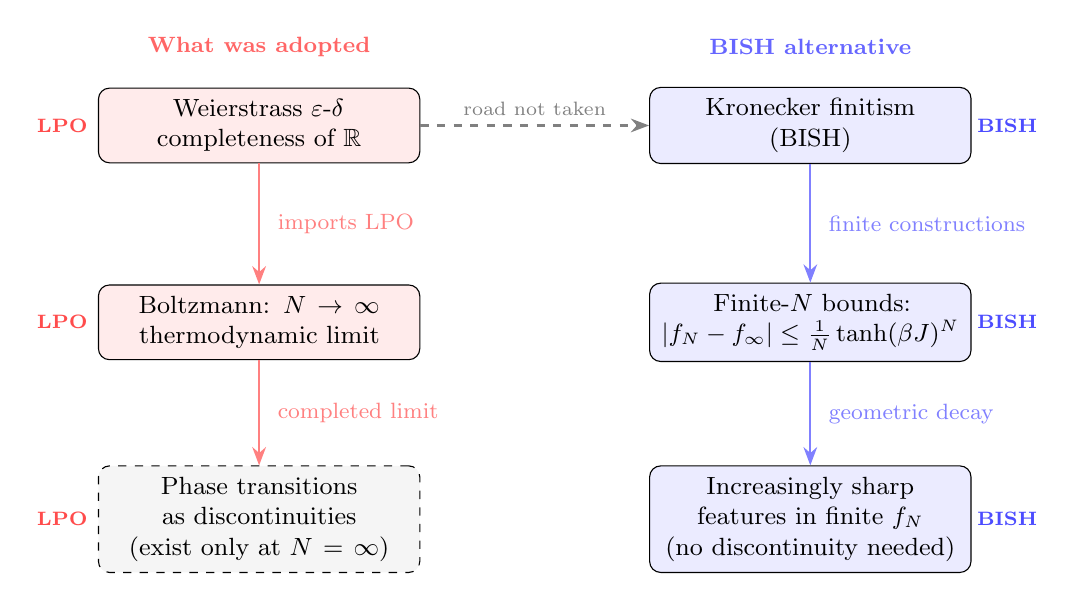
\begin{tikzpicture}[
  >=Stealth,
  every node/.style={font=\small},
  box/.style={draw, rounded corners, minimum height=0.9cm, text width=3.8cm, align=center, inner sep=4pt},
  adopted/.style={box, fill=red!8},
  bish/.style={box, fill=blue!8},
  result/.style={box, fill=gray!8, dashed},
  lbl/.style={font=\footnotesize, midway, right=3pt}
]
% Left column: what was adopted
\node[adopted] (weier) at (0, 5.0) {Weierstrass $\varepsilon$-$\delta$\\completeness of $\mathbb{R}$};
\node[adopted] (boltz) at (0, 2.5) {Boltzmann: $N \to \infty$\\thermodynamic limit};
\node[result] (phase) at (0, 0) {Phase transitions\\as discontinuities\\(exist only at $N = \infty$)};

% Right column: BISH alternative
\node[bish] (kron) at (7, 5.0) {Kronecker finitism\\(BISH)};
\node[bish] (finite) at (7, 2.5) {Finite-$N$ bounds:\\$|f_N - f_\infty| \leq \frac{1}{N}\tanh(\beta J)^N$};
\node[bish] (sharp) at (7, 0) {Increasingly sharp\\features in finite $f_N$\\(no discontinuity needed)};

% Arrows left column
\draw[->, thick, red!50] (weier) -- node[lbl] {imports LPO} (boltz);
\draw[->, thick, red!50] (boltz) -- node[lbl] {completed limit} (phase);

% Arrows right column
\draw[->, thick, blue!50] (kron) -- node[lbl] {finite constructions} (finite);
\draw[->, thick, blue!50] (finite) -- node[lbl] {geometric decay} (sharp);

% Cross arrows
\draw[->, thick, dashed, gray] (weier) -- node[above, font=\scriptsize] {road not taken} (kron);

% Labels
\node[font=\footnotesize\bfseries, red!60] at (0, 6.0) {What was adopted};
\node[font=\footnotesize\bfseries, blue!60] at (7, 6.0) {BISH alternative};

% Cost labels
\node[font=\scriptsize\bfseries, red!70] at (-2.5, 5.0) {LPO};
\node[font=\scriptsize\bfseries, red!70] at (-2.5, 2.5) {LPO};
\node[font=\scriptsize\bfseries, red!70] at (-2.5, 0) {LPO};
\node[font=\scriptsize\bfseries, blue!70] at (9.5, 5.0) {BISH};
\node[font=\scriptsize\bfseries, blue!70] at (9.5, 2.5) {BISH};
\node[font=\scriptsize\bfseries, blue!70] at (9.5, 0) {BISH};

\end{tikzpicture}
\caption{Act~I: the Weierstrass--Boltzmann import.
Weierstrass's completeness of the reals (LPO) was inherited by Boltzmann's thermodynamic limit.
The BISH alternative---finite-$N$ error bounds with geometric decay---recovers every empirical prediction without the completed limit.
The ``road not taken'' from Kronecker finitism was available from the 1870s.}
\label{fig:act1-import}
\end{figure}

% ============================================================
\section{Act~II: The Quantum Formalization (1925--1935)}
% ============================================================

Quantum mechanics was born constructive and became classical.

Heisenberg's matrix mechanics (1925) was intrinsically finite-dimensional and algebraic.
Matrices, commutators, trace formulas---the operational toolkit of quantum mechanics is linear algebra, and finite-dimensional linear algebra is BISH to the core.
Schr\"odinger's wave mechanics (1926) introduced infinite-dimensional function spaces, but the actual calculations---the hydrogen atom, the harmonic oscillator---used finite-term power series and explicit formulas.
Dirac's transformation theory (1927) unified matrix and wave mechanics through a powerful notation that also obscured the question of dimension.

A scope note is necessary here.
The constructive calibration programme examines quantum \emph{states}---density matrices, singular states, spectral structure---not quantum \emph{dynamics}.
Time evolution operators, scattering amplitudes, the S-matrix, and path integrals for dynamical processes remain uncalibrated.
The results below concern the static mathematical objects of quantum theory, not the dynamical ones.

Then came von~Neumann.

In 1932, von~Neumann published \emph{Mathematische Grundlagen der Quantenmechanik} \cite{vonNeumann1932}, which axiomatized quantum mechanics in terms of infinite-dimensional Hilbert spaces, the spectral theorem for unbounded self-adjoint operators, and the theory of von~Neumann algebras.
This was a masterwork of mathematical architecture---and a consequential trade.
A finite, operational physical theory was recast in the language of infinite-dimensional functional analysis, gaining enormous conceptual power (general spectral theory, representation theory, the classification of quantum symmetries) at a logical cost that would remain invisible for ninety years.
The physics community gained a thinking tool of extraordinary scope and gradually lost the ability to distinguish the physics from the tool.

Our programme reveals the cost.
The Heisenberg uncertainty principle---arguably the defining statement of quantum mechanics---splits into two logically distinct results \cite{Lee2026g}.
The \emph{preparation uncertainty} inequality (the Robertson-Schr\"odinger bound) states that for any quantum state~$\psi$ with $\|\psi\|=1$ and any pair of observables $A$, $B$:
\begin{equation}\label{eq:rs-inequality}
|\langle \psi, [A,B]\,\psi\rangle|^2 \;\leq\; 4\,\mathrm{Var}_\psi(A)\;\mathrm{Var}_\psi(B),
\end{equation}
where $\mathrm{Var}_\psi(A) = \|A\psi - \langle A\rangle\psi\|^2$ and $[A,B] = AB - BA$.
This is fully constructive: the proof centers the state, applies the Cauchy-Schwarz inequality to the inner product $\langle \Delta_A\psi, \Delta_B\psi\rangle$, and decomposes the result into commutator and anticommutator contributions.
Pure Hilbert space geometry---BISH.
The \emph{measurement uncertainty} form---which concerns the statistics extracted from repeated measurements---requires Dependent Choice, a modest extension that allows countable sequences of dependent selections.
The physical core of quantum uncertainty needs no classical logic.
The classical overhead enters only when you extract statistical information from infinite measurement sequences.

This separation has a deeper significance than a technical footnote about choice principles.
The Born rule---the postulate that measurement probabilities equal $|\langle\lambda|\psi\rangle|^2$---is itself an idealization.
It asserts that relative frequencies over infinitely many measurements converge to definite probabilities; that convergence is where Dependent Choice enters.
The geometric content of quantum mechanics---that a single state cannot be simultaneously sharp in non-commuting observables---is BISH, a property of one vector in a finite-dimensional Hilbert space requiring no measurements at all.
The statistical content---that repeated measurements yield frequencies approaching the Born probabilities---requires the construction of infinite measurement sequences and the extraction of their limits.
Quantum mechanics thus splits into two logical layers: a constructive geometric core (preparation uncertainty, Cauchy--Schwarz, BISH) and a statistical superstructure (measurement uncertainty, the Born rule, Dependent Choice).
The physical core that makes quantum mechanics \emph{strange}---superposition, interference, non-commutativity---needs no idealization.
The apparatus that makes quantum mechanics \emph{predictive} over infinite ensembles does.

\begin{figure}[ht]
\centering
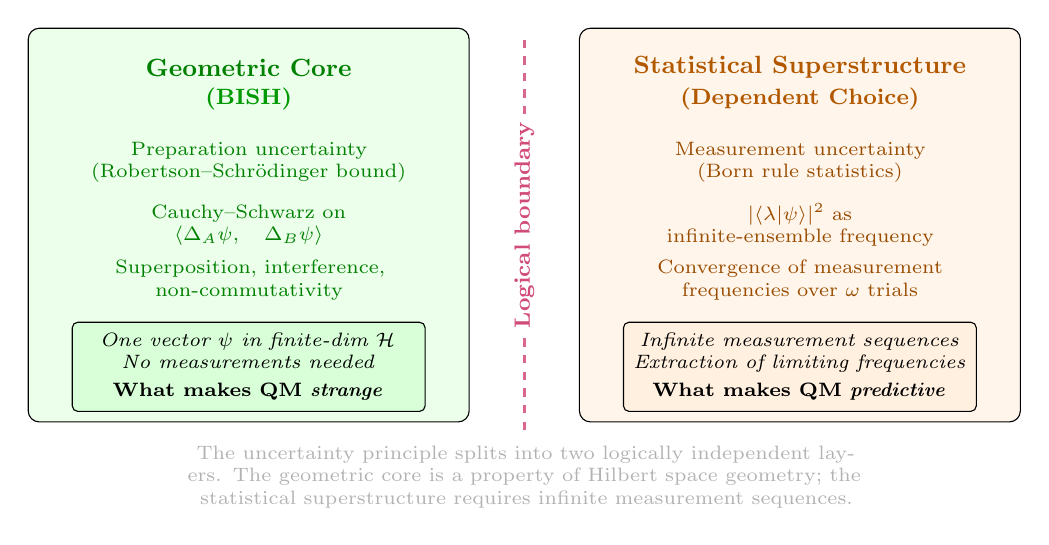
\begin{tikzpicture}[
  >=Stealth,
  every node/.style={font=\small},
  panel/.style={draw, rounded corners=4pt, minimum width=5.6cm,
                minimum height=5.0cm, align=center, inner sep=6pt}
]
% ---- LEFT PANEL: Geometric Core (BISH) ----
\node[panel, fill=green!8] (geo) at (-3.5, 0) {};
\node[font=\small\bfseries, green!50!black] at (-3.5, 2.0)
  {Geometric Core};
\node[font=\footnotesize\bfseries, green!60!black] at (-3.5, 1.6)
  {(BISH)};

% Content items
\node[font=\scriptsize, green!50!black, text width=4.5cm, align=center]
  at (-3.5, 0.8) {Preparation uncertainty\\(Robertson--Schr\"odinger bound)};
\node[font=\scriptsize, green!50!black, text width=4.5cm, align=center]
  at (-3.5, 0.0) {Cauchy--Schwarz on\\$\langle\Delta_A\psi,\;\Delta_B\psi\rangle$};
\node[font=\scriptsize, green!50!black, text width=4.5cm, align=center]
  at (-3.5, -0.7) {Superposition, interference,\\non-commutativity};

% Bottom annotation
\node[draw, rounded corners=2pt, fill=green!15,
      font=\scriptsize\itshape, text width=4.2cm, align=center,
      inner sep=4pt]
  at (-3.5, -1.8) {One vector $\psi$ in finite-dim $\mathcal{H}$\\
  No measurements needed\\[2pt]
  \upshape\textbf{What makes QM \emph{strange}}};

% ---- RIGHT PANEL: Statistical Superstructure (DC) ----
\node[panel, fill=orange!8] (stat) at (3.5, 0) {};
\node[font=\small\bfseries, orange!70!black] at (3.5, 2.0)
  {Statistical Superstructure};
\node[font=\footnotesize\bfseries, orange!70!black] at (3.5, 1.6)
  {(Dependent Choice)};

% Content items
\node[font=\scriptsize, orange!60!black, text width=4.5cm, align=center]
  at (3.5, 0.8) {Measurement uncertainty\\(Born rule statistics)};
\node[font=\scriptsize, orange!60!black, text width=4.5cm, align=center]
  at (3.5, 0.0) {$|\langle\lambda|\psi\rangle|^2$ as\\
  infinite-ensemble frequency};
\node[font=\scriptsize, orange!60!black, text width=4.5cm, align=center]
  at (3.5, -0.7) {Convergence of measurement\\frequencies over $\omega$ trials};

% Bottom annotation
\node[draw, rounded corners=2pt, fill=orange!12,
      font=\scriptsize\itshape, text width=4.2cm, align=center,
      inner sep=4pt]
  at (3.5, -1.8) {Infinite measurement sequences\\
  Extraction of limiting frequencies\\[2pt]
  \upshape\textbf{What makes QM \emph{predictive}}};

% ---- CENTRAL BOUNDARY ----
\draw[very thick, purple!60, dashed] (0, -2.6) -- (0, 2.4);
\node[font=\footnotesize\bfseries, purple!70, fill=white,
      inner sep=3pt, rotate=90]
  at (0, 0) {Logical boundary};

% ---- BOTTOM ANNOTATION ----
\node[font=\scriptsize, gray!60, text width=10cm, align=center]
  at (0, -3.2)
  {The uncertainty principle splits into two logically independent layers.
  The geometric core is a property of Hilbert space geometry;
  the statistical superstructure requires infinite measurement sequences.};

\end{tikzpicture}
\caption{The Heisenberg split.
The uncertainty principle decomposes into two logically independent components:
a constructive geometric core (preparation uncertainty, Cauchy--Schwarz, BISH)
and a statistical superstructure (measurement uncertainty, the Born rule,
Dependent Choice).
The physical content that makes quantum mechanics \emph{strange} requires no
idealization; the apparatus that makes it \emph{predictive} over infinite
ensembles does.}
\label{fig:heisenberg-split}
\end{figure}

The distinction between physical states and mathematical artifacts is even sharper.
In quantum mechanics, physical states are represented by density matrices---positive operators of unit trace on the Hilbert space.
But the mathematical dual of the trace-class operators contains objects that are \emph{not} density matrices: the \emph{singular states}, functionals that vanish on all compact operators and detect only behavior at spatial infinity.
No laboratory has ever prepared a singular state, because doing so would require controlling infinitely many degrees of freedom simultaneously.

Our programme shows that the mere non-reflexivity of the state space---the fact that singular states ``cannot be ruled out''---is provable in BISH \cite{Lee2026b}.
But \emph{constructively exhibiting} a singular state, with explicit separation data from the space of density matrices, requires WLPO \cite{Lee2026a}.
The gap between ``cannot rule out'' and ``can exhibit'' is precisely the WLPO boundary.
Singular states are cities that appear on the map but have no corresponding settlement in the territory.

Most strikingly, the research programme establishes that Bell nonlocality---the phenomenon that makes quantum mechanics genuinely non-classical---requires no classical logic at all \cite{Lee2026paper11}.
The Tsirelson bound on the CHSH correlations decomposes algebraically: define the CHSH operator
\begin{equation}\label{eq:chsh}
\mathcal{C} \;=\; A \otimes (B + B') \;+\; A' \otimes (B - B')
\end{equation}
where $A, A', B, B'$ are self-adjoint involutions ($A^2 = I$, etc.)\ on $\mathbb{C}^2$.
Because involutions preserve norms, $\|\mathcal{C}\psi\|^2 \leq \|(B+B')\psi_B\|^2 + \|(B-B')\psi_B\|^2$, and the identity $(B+B')^2 + (B-B')^2 = 4I$ yields:
\[
|\langle \psi, \mathcal{C}\psi\rangle| \;\leq\; 2\sqrt{2}.
\]
This is the Tsirelson bound---a theorem of finite-dimensional linear algebra: $4\times 4$ matrices, a sum-of-squares identity, and the parallelogram inequality.
The proof is BISH.
The most distinctively quantum phenomenon needs the least logical strength.

The spectrum itself---the central mathematical object of quantum mechanics, the set of possible measurement outcomes for an observable---is an idealization.
An experimentalist measures finitely many energy levels to finite precision: the hydrogen Lyman series, a handful of absorption lines, each located within instrumental error bars.
That is BISH\@.
The assertion that a specific value $\lambda$ belongs \emph{exactly} to the spectrum of an operator~$H$---rather than merely within~$\varepsilon$ of the spectrum for every~$\varepsilon > 0$---requires Markov's Principle \cite{Lee2026f}.
The full spectral theorem, guaranteeing a complete projection-valued measure decomposing any self-adjoint operator into spectral subspaces, requires substantially more.
The most fundamental mathematical structure of quantum mechanics---the object from which every measurement prediction flows---has a precisely calibrated logical cost, and the physical content accessible to a finite observer sits below that cost at BISH\@.

Taken together, the quantum calibrations reveal a layered architecture.
Von~Neumann's 1932 formalization introduced not one but three measurable layers of idealization above BISH: the Born rule's convergence of measurement statistics (Dependent Choice, \cite{Lee2026g}), exact spectral membership (Markov's Principle, \cite{Lee2026f}), and the existence of singular states in the bidual (WLPO, \cite{Lee2026a}).
Each layer has a machine-verified logical cost.
Each separates physical content from mathematical infrastructure.
The pattern is uniform: what a finite observer can prepare, measure, and record is BISH; each assertion about completed infinities---infinite measurement sequences, exact set membership, functionals on infinite-dimensional duals---costs a specific, independently identifiable non-constructive principle.

\begin{figure}[ht]
\centering
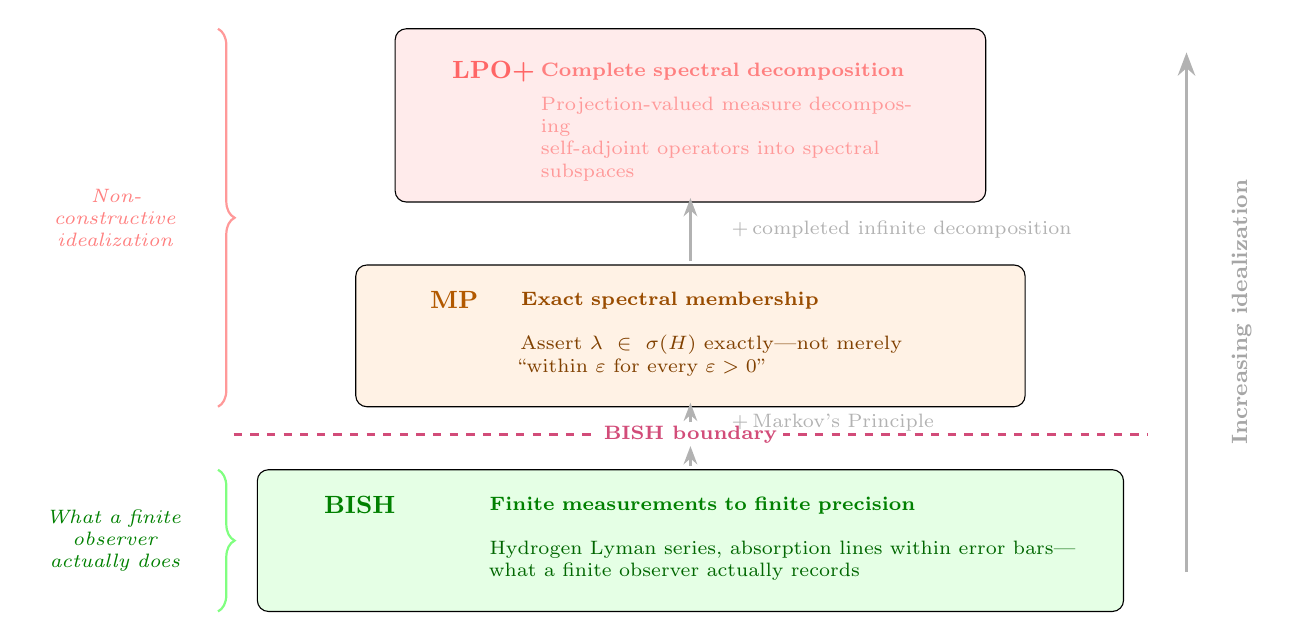
\begin{tikzpicture}[
  >=Stealth,
  every node/.style={font=\small}
]
% ---- BOTTOM: BISH (finite measurements) — widest ----
\node[draw, rounded corners=4pt, minimum width=11cm,
      minimum height=1.8cm, fill=green!10] (bish) at (0, 0) {};
\node[font=\small\bfseries, green!50!black] at (-4.2, 0.45)
  {BISH};
\node[font=\scriptsize, green!50!black, text width=7.5cm, align=left]
  at (1.2, 0.45) {\textbf{Finite measurements to finite precision}};
\node[font=\scriptsize, green!40!black, text width=7.5cm, align=left]
  at (1.2, -0.25) {Hydrogen Lyman series, absorption lines within
  error bars---\\what a finite observer actually records};

% ---- MIDDLE: Markov's Principle — narrower ----
\node[draw, rounded corners=4pt, minimum width=8.5cm,
      minimum height=1.8cm, fill=orange!10] (mp) at (0, 2.6) {};
\node[font=\small\bfseries, orange!70!black] at (-3.0, 3.05)
  {MP};
\node[font=\scriptsize, orange!60!black, text width=5.5cm, align=left]
  at (0.6, 3.05) {\textbf{Exact spectral membership}};
\node[font=\scriptsize, orange!50!black, text width=5.5cm, align=left]
  at (0.6, 2.35) {Assert $\lambda \in \sigma(H)$ exactly---not merely
  ``within $\varepsilon$ for every $\varepsilon > 0$''};

% ---- TOP: Full spectral theorem — narrowest ----
\node[draw, rounded corners=4pt, minimum width=7.5cm,
      minimum height=2.2cm, fill=red!8] (full) at (0, 5.4) {};
\node[font=\small\bfseries, red!60] at (-2.5, 5.95)
  {LPO+};
\node[font=\scriptsize, red!50, text width=4.8cm, align=left]
  at (0.5, 5.95) {\textbf{Complete spectral decomposition}};
\node[font=\scriptsize, red!40, text width=4.8cm, align=left]
  at (0.5, 5.1) {Projection-valued measure decomposing\\self-adjoint operators into spectral subspaces};

% ---- BISH BOUNDARY ----
\draw[very thick, dashed, purple!70] (-5.8, 1.35) -- (5.8, 1.35);
\node[font=\scriptsize\bfseries, purple!70, fill=white, inner sep=2pt]
  at (0, 1.35) {BISH boundary};

% ---- ARROWS between levels ----
\draw[->, thick, gray!60] (0, 0.95) -- (0, 1.2);
\draw[->, thick, gray!60] (0, 1.5) -- (0, 1.75);
\node[font=\scriptsize, gray!60, anchor=west] at (0.4, 1.5)
  {+\,Markov's Principle};
\draw[->, thick, gray!60] (0, 3.55) -- (0, 4.35);
\node[font=\scriptsize, gray!60, anchor=west] at (0.4, 3.95)
  {+\,completed infinite decomposition};

% ---- RIGHT ARROW: idealization axis ----
\draw[->, very thick, gray!60] (6.3, -0.4) -- (6.3, 6.2);
\node[font=\footnotesize\bfseries, gray!70, rotate=90] at (7.0, 2.9)
  {Increasing idealization};

% ---- LEFT brace: finite observer ----
\draw[thick, green!50, decorate,
      decoration={brace, amplitude=6pt, mirror}]
  (-6.0, -0.9) -- (-6.0, 0.9);
\node[font=\scriptsize\itshape, green!50!black, text width=2cm,
      align=center]
  at (-7.3, 0) {What a finite\\observer\\actually does};

% ---- LEFT brace: non-constructive idealization ----
\draw[thick, red!40, decorate,
      decoration={brace, amplitude=6pt, mirror}]
  (-6.0, 1.7) -- (-6.0, 6.5);
\node[font=\scriptsize\itshape, red!50, text width=2cm,
      align=center]
  at (-7.3, 4.1) {Non-constructive\\idealization};

\end{tikzpicture}
\caption{The spectrum as idealization.
The quantum spectrum has three levels of logical cost.
A finite observer measures finitely many energy levels to finite
precision (BISH, bottom).
Asserting exact spectral membership costs Markov's Principle (middle).
The full spectral decomposition, from which all textbook predictions
formally flow, requires substantially more (top).
The physical content accessible to experiment sits at the bottom.}
\label{fig:spectrum-idealization}
\end{figure}

\textbf{The constructive alternative.}
It was not merely available---it was actively contested.
Brouwer's intuitionism was at its most creative precisely during the decade (1920--1930) when quantum mechanics was being formalized.
In 1928, the year Dirac published his equation and von~Neumann began his axiomatization, Hilbert had Brouwer expelled from the editorial board of \emph{Mathematische Annalen}---marginalizing intuitionism at the very moment the quantum formalism was hardening \cite{vanDalen2005}.
A decade earlier, Hermann Weyl had published \emph{Das Kontinuum} (1918) \cite{Weyl1918}, constructing a predicative foundation for analysis explicitly intended for physical application.
Weyl abandoned this programme under social pressure from the Hilbert school, not because of any mathematical inadequacy.
Most remarkably, von~Neumann himself grew dissatisfied with the Hilbert space formalism within a few years and turned to finite type~II$_1$ factors---where the pathologies of unbounded operators and non-reflexivity vanish \cite{Redei1996}.
The architect of the cathedral privately preferred the cellar.

\begin{figure}[ht]
\centering
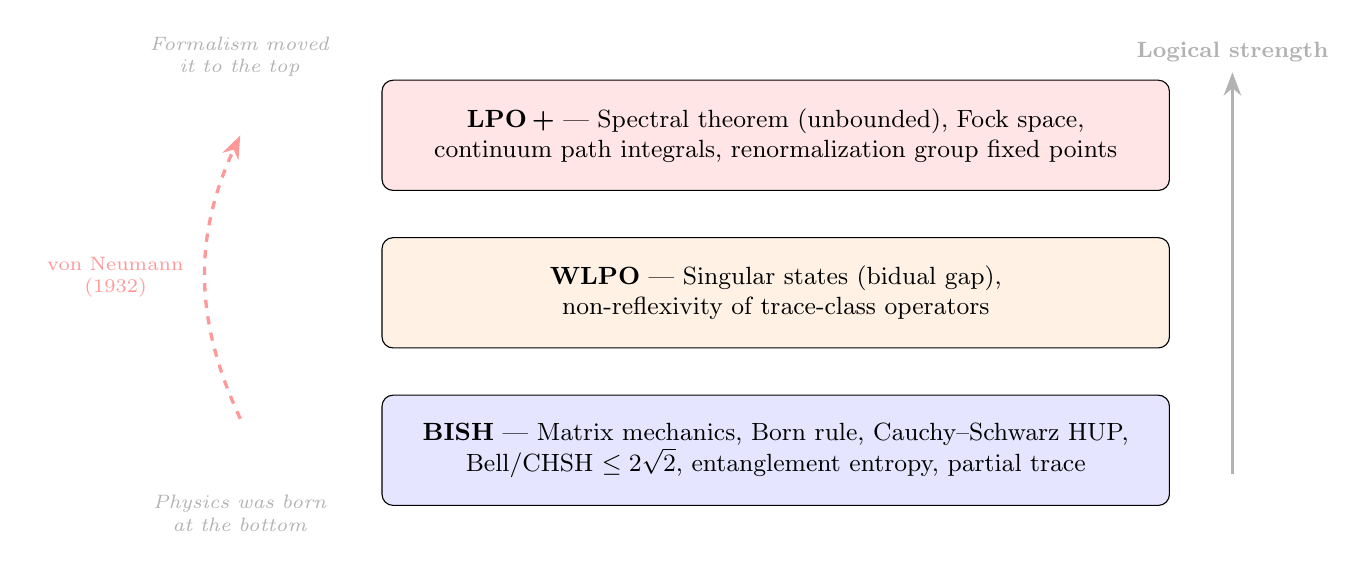
\begin{tikzpicture}[
  >=Stealth,
  every node/.style={font=\small},
  layer/.style={draw, minimum width=10cm, minimum height=1.4cm, align=center, inner sep=4pt}
]
% Bottom layer: BISH
\node[layer, fill=blue!10, rounded corners] (bish) at (0, 0)
  {\textbf{BISH} --- Matrix mechanics, Born rule, Cauchy--Schwarz HUP,\\
   Bell/CHSH $\leq 2\sqrt{2}$, entanglement entropy, partial trace};
% Middle layer: WLPO
\node[layer, fill=orange!10, rounded corners] (wlpo) at (0, 2)
  {\textbf{WLPO} --- Singular states (bidual gap),\\
   non-reflexivity of trace-class operators};
% Top layer: LPO+
\node[layer, fill=red!10, rounded corners] (lpo) at (0, 4)
  {\textbf{LPO\,+} --- Spectral theorem (unbounded), Fock space,\\
   continuum path integrals, renormalization group fixed points};

% Arrow on right
\draw[->, very thick, gray!60] (5.8, -0.3) -- (5.8, 4.8)
  node[above, font=\footnotesize\bfseries, gray!60] {Logical strength};

% Von Neumann arrow
\draw[->, very thick, red!40, dashed] (-6.8, 0.4) to[bend left=25]
  node[left, font=\scriptsize, text width=2cm, align=center] {von Neumann\\(1932)} (-6.8, 4.0);

% Annotation
\node[font=\scriptsize\itshape, gray!60, text width=3cm, align=center] at (-6.8, -0.8)
  {Physics was born\\at the bottom};
\node[font=\scriptsize\itshape, gray!60, text width=3cm, align=center] at (-6.8, 5.0)
  {Formalism moved\\it to the top};

\end{tikzpicture}
\caption{Act~II: the quantum formalization.
Heisenberg's matrix mechanics (1925) is BISH\@.
Von~Neumann's Hilbert space axiomatization (1932) moved the formalism to infinite dimensions.
The empirical content---uncertainty relations, Bell nonlocality, entanglement entropy---remains at BISH\@.
Singular states (WLPO) are mathematical artifacts of the infinite-dimensional framework.}
\label{fig:quantum-layers}
\end{figure}

\begin{keymessage}
Quantum mechanics was born constructive (matrix mechanics = BISH).
Von~Neumann moved it to infinite dimensions (1932).
The HUP, Bell/CHSH, and entanglement entropy are all BISH; singular states cost WLPO\@.
The empirical content stayed at sea level; only the formalism ascended.
\end{keymessage}

% ============================================================
\section{Act~III: The Singularity Detour (1939--1970)}
% ============================================================

In 1939, Einstein published a paper arguing that gravitational collapse could not produce singularities---points of infinite curvature where the equations of general relativity break down \cite{Einstein1939}.
His conviction was principled: ``Every field theory, in our opinion, must therefore adhere to the fundamental principle that singularities of the field are to be excluded.''
Infinite curvature at a point, he reasoned, is not something the physical world produces.
It is a mathematical pathology, an artifact of pushing the formalism past its domain of validity.

The same year, Oppenheimer and Snyder published a paper showing that for a sufficiently massive star, gravitational collapse is inevitable \cite{OppenheimerSnyder1939}.
The community sided with Oppenheimer.
Then, in 1965, Penrose proved the first singularity theorem \cite{Penrose1965}: under generic conditions---trapped surfaces, reasonable energy conditions, global hyperbolicity---spacetime is geodesically incomplete.
Incomplete geodesics are the mathematical signature of singularities.
Hawking extended the result, and the Hawking-Penrose theorems (1970) established singularities as an inescapable feature of general relativity.
Einstein, who died in 1955, was posthumously declared wrong.

Our framework reaches a conclusion that aligns with his, though for entirely different reasons he could not have articulated.
His 1939 argument was physically flawed---it relied on circular orbit stability, which is irrelevant to radial collapse---but his conclusion that singularities are artifacts of the formalism rather than features of the world aligns with the constructive verdict, which locates the artifact precisely at the LPO boundary.

The Penrose singularity theorem has the following logical structure.
The Raychaudhuri equation \cite{Raychaudhuri1955} governs the evolution of the expansion scalar $\theta$ along a geodesic congruence:
\begin{equation}\label{eq:raychaudhuri}
\frac{d\theta}{d\tau} \;=\; -\frac{1}{3}\theta^2 \;-\; \sigma_{\mu\nu}\sigma^{\mu\nu} \;+\; \omega_{\mu\nu}\omega^{\mu\nu} \;-\; R_{\mu\nu}\,u^\mu u^\nu,
\end{equation}
where $\sigma_{\mu\nu}$ is the shear tensor, $\omega_{\mu\nu}$ is the vorticity, $R_{\mu\nu}$ is the Ricci tensor, and $u^\mu$ is the tangent vector.
When the strong energy condition holds ($R_{\mu\nu}u^\mu u^\nu \geq 0$) and vorticity vanishes, the right-hand side is non-positive: the expansion decreases monotonically.
This is a first-order ordinary differential equation on finite parameter intervals---\emph{BISH}.
(The equation displayed is the \emph{timelike} Raychaudhuri equation; Penrose's 1965 theorem uses the \emph{null} version, with $\tfrac{1}{2}\theta^2$ replacing $\tfrac{1}{3}\theta^2$ and vanishing vorticity guaranteed by the twist-free hypothesis on the null geodesic congruence.
The logical structure---finite ODE at BISH, completed limit at LPO---is identical in both cases.)

The non-constructive step comes at the end, and it is the same step as in the thermodynamic limit.
The Penrose theorem asserts a dichotomy on the monotonically decreasing expansion scalar: either the geodesic terminates at finite parameter value (singularity) or it extends forever.
This is Bounded Monotone Convergence---LPO \cite{BridgesVita2006}.
The physical content of the singularity theorem is the Raychaudhuri focusing, which is BISH.
The Kretschmann curvature invariant $K = 48M^2/r^6$ is constructively computable for any $r > 0$, and its divergence is constructively witnessable: for any bound~$B$, one can constructively exhibit~$r_0 > 0$ with $K(r_0) > B$.
This unbounded growth is BISH---not a completed limit.
The completed-limit content resides in the assertion that the geodesic actually \emph{reaches} $r = 0$: that a bounded monotone decreasing sequence of radial coordinates converges to a definite real number.
This is the same bounded monotone convergence equivalence (BMC~$\equiv$~LPO) as in the thermodynamic limit \cite{Lee2026paper13}.
The physics is the focusing; the singularity is where the map says ``here be dragons.''
The territory just keeps going.

Paper~13 \cite{Lee2026paper13} formalizes this decomposition for the Schwarzschild case.
The event horizon at $r = 2M$ serves as a \emph{logical boundary}: the exterior geometry (Paper~1) and the interior's finite-time physics---the cycloid geodesic reaching $r = 0$ at proper time $\tau^* = \pi M$, the Kretschmann scalar's constructively witnessable divergence---are BISH.
Only the completed-limit assertion that every bounded monotone trajectory converges to a definite real costs LPO.
The horizon demarcates what can be asserted without surveying an infinite set.

\textbf{The constructive alternative.}
Einstein was not alone in his discomfort.
Eddington found singularities ``repugnant'' and publicly attacked Chandrasekhar's mass limit calculations in 1935.
The Raychaudhuri equation itself---the constructive core of the singularity theorems---provides all the physical content: quantitative bounds on geodesic convergence over finite parameter intervals.
Every numerical relativity simulation operates at this BISH level, computing finite-precision approximations to geodesic behavior without asserting completed limits---from binary black hole merger simulations to gravitational wave template generation, all finite-precision computations on finite grids.
As recently as 2023, Roy Kerr---discoverer of the Kerr metric for rotating black holes---has argued that physical black holes need not contain singularities \cite{Kerr2023}.
The constructive verdict aligns with a persistent minority view in general relativity: the physics is the focusing, and the singularity is the idealization.

\begin{figure}[ht]
\centering
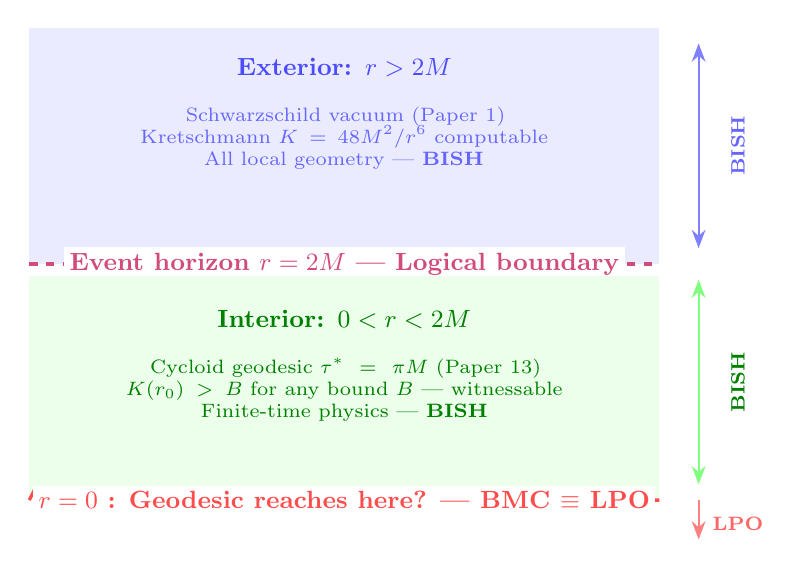
\begin{tikzpicture}[
  >=Stealth,
  every node/.style={font=\small}
]
% Exterior region
\fill[blue!8] (-4, 0) rectangle (4, 3);
\node[font=\small\bfseries, blue!70] at (0, 2.5) {Exterior: $r > 2M$};
\node[font=\scriptsize, blue!60, text width=6cm, align=center] at (0, 1.6)
  {Schwarzschild vacuum (Paper~1)\\Kretschmann $K = 48M^2/r^6$ computable\\All local geometry --- \textbf{BISH}};

% Event horizon
\draw[very thick, dashed, purple!70] (-4, 0) -- (4, 0);
\node[font=\small\bfseries, purple!70, fill=white, inner sep=2pt] at (0, 0) {Event horizon $r = 2M$ --- Logical boundary};

% Interior region
\fill[green!8] (-4, -3) rectangle (4, -0.15);
\node[font=\small\bfseries, green!50!black] at (0, -0.7) {Interior: $0 < r < 2M$};
\node[font=\scriptsize, green!50!black, text width=6.5cm, align=center] at (0, -1.6)
  {Cycloid geodesic $\tau^* = \pi M$ (Paper~13)\\$K(r_0) > B$ for any bound $B$ --- witnessable\\Finite-time physics --- \textbf{BISH}};

% Singularity
\draw[very thick, red!70, decorate, decoration={zigzag, segment length=6pt, amplitude=3pt}]
  (-4, -3) -- (4, -3);
\node[font=\small\bfseries, red!70, fill=white, inner sep=2pt] at (0, -3)
  {$r = 0$ : Geodesic reaches here? --- \textbf{BMC $\equiv$ LPO}};

% Right-side labels
\draw[thick, blue!50, <->] (4.5, 0.2) -- (4.5, 2.8);
\node[font=\scriptsize\bfseries, blue!60, rotate=90] at (5.0, 1.5) {BISH};
\draw[thick, green!50, <->] (4.5, -2.8) -- (4.5, -0.2);
\node[font=\scriptsize\bfseries, green!50!black, rotate=90] at (5.0, -1.5) {BISH};
\draw[thick, red!50, ->] (4.5, -3.0) -- (4.5, -3.5);
\node[font=\scriptsize\bfseries, red!60] at (5.0, -3.3) {LPO};

\end{tikzpicture}
\caption{Act~III: the event horizon as a logical boundary.
The exterior geometry and the interior's finite-time physics are both BISH\@.
The singularity---the assertion that a bounded monotone trajectory converges to a definite real---costs LPO\@.
The horizon demarcates what can be asserted without surveying an infinite set (Paper~13).}
\label{fig:blackhole}
\end{figure}

\begin{figure}[ht]
\centering
\resizebox{\textwidth}{!}{%
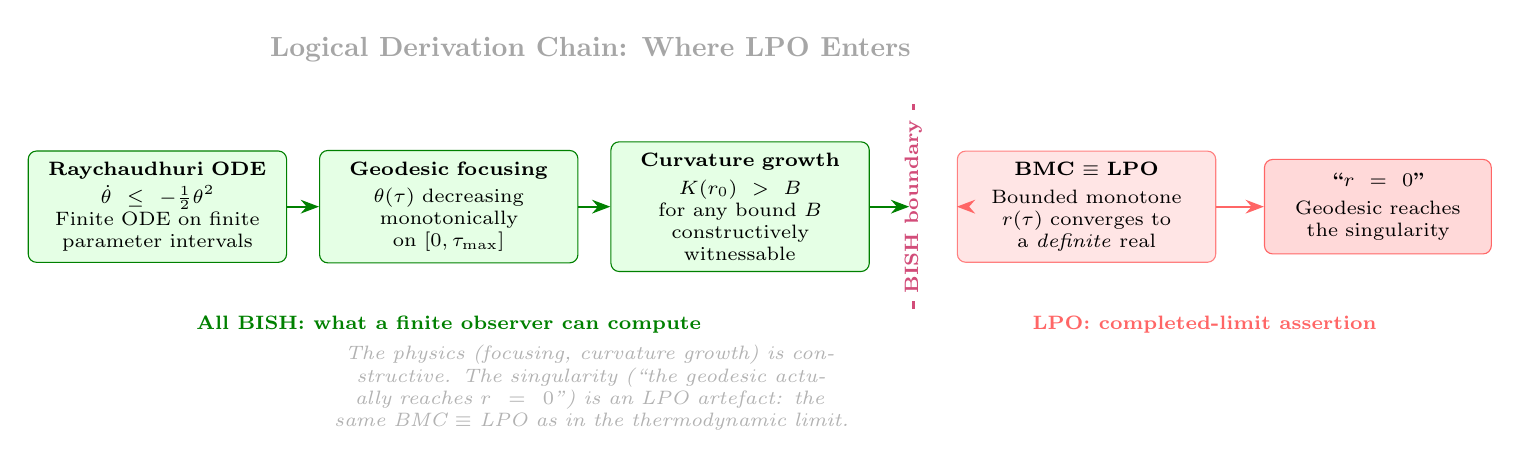
\begin{tikzpicture}[
  >=Stealth,
  every node/.style={font=\small},
  chainbox/.style={draw, rounded corners=3pt, font=\scriptsize,
               minimum height=1.2cm, text width=3.0cm, align=center,
               inner sep=4pt},
  lpostep/.style={chainbox, fill=red!10, draw=red!50},
  bishstep/.style={chainbox, fill=green!10, draw=green!50!black}
]
% ---- Title ----
\node[font=\normalsize\bfseries, gray!70] at (5.5, 3.2)
  {Logical Derivation Chain: Where LPO Enters};

% ---- BISH steps (left to right) ----
\node[bishstep] (ray) at (0, 1.2)
  {\textbf{Raychaudhuri ODE}\\[2pt]$\dot\theta \leq -\tfrac{1}{2}\theta^2$\\
   Finite ODE on finite\\parameter intervals};

\node[bishstep] (focus) at (3.7, 1.2)
  {\textbf{Geodesic focusing}\\[2pt]$\theta(\tau)$ decreasing\\monotonically\\on $[0, \tau_{\max}]$};

\node[bishstep] (curv) at (7.4, 1.2)
  {\textbf{Curvature growth}\\[2pt]$K(r_0) > B$\\for any bound $B$\\constructively witnessable};

% ---- BISH boundary ----
\draw[very thick, dashed, purple!70] (9.6, -0.1) -- (9.6, 2.5);
\node[font=\scriptsize\bfseries, purple!70, fill=white, inner sep=2pt,
      rotate=90] at (9.6, 1.2) {BISH boundary};

% ---- LPO step ----
\node[lpostep] (bmc) at (11.8, 1.2)
  {\textbf{BMC $\equiv$ LPO}\\[2pt]Bounded monotone\\$r(\tau)$ converges to\\a \emph{definite} real};

% ---- Conclusion ----
\node[draw, rounded corners=3pt, fill=red!15, draw=red!60,
      font=\scriptsize, minimum height=1.2cm, text width=2.6cm,
      align=center, inner sep=4pt] (sing) at (15.5, 1.2)
  {\textbf{``$r = 0$''}\\[2pt]Geodesic reaches\\the singularity};

% ---- Arrows ----
\draw[->, thick, green!50!black] (ray.east) -- (focus.west);
\draw[->, thick, green!50!black] (focus.east) -- (curv.west);
\draw[->, thick, green!50!black] (curv.east) -- ++(0.5, 0);
\draw[->, thick, red!60] (10.2, 1.2) -- (bmc.west);
\draw[->, thick, red!60] (bmc.east) -- (sing.west);

% ---- Labels below ----
\node[font=\scriptsize\bfseries, green!50!black] at (3.7, -0.3)
  {All BISH: what a finite observer can compute};
\node[font=\scriptsize\bfseries, red!60] at (13.3, -0.3)
  {LPO: completed-limit assertion};

% ---- Annotation ----
\node[font=\scriptsize\itshape, gray!60, text width=8cm, align=center]
  at (5.5, -1.1)
  {The physics (focusing, curvature growth) is constructive.
   The singularity (``the geodesic actually reaches $r=0$'') is an LPO artefact:
   the same BMC~$\equiv$~LPO as in the thermodynamic limit.};

\end{tikzpicture}%
}%
\caption{The logical derivation chain for Schwarzschild geodesic incompleteness (exemplifying the Penrose pattern).
The Raychaudhuri equation, geodesic focusing, and curvature growth are all BISH---finite
ODEs on finite parameter intervals.
The non-constructive step is Bounded Monotone Convergence (BMC~$\equiv$~LPO):
the assertion that the bounded monotone radial coordinate sequence converges to a definite real.
This is the same LPO cost that governs the thermodynamic limit (Paper~8), confirming
domain invariance of the logical cost.}
\label{fig:singularity-chain}
\end{figure}

\begin{keymessage}
The Raychaudhuri focusing equation is BISH\@.
The Kretschmann divergence is constructively witnessable.
Only the assertion ``the geodesic reaches $r = 0$'' costs LPO---the same BMC equivalence as the thermodynamic limit.
The event horizon is a logical boundary (Paper~13).
\end{keymessage}

% ============================================================
\section{Act~IV: The Greatest Predictions from the Smallest Logic (1947--1975)}
% ============================================================

Between 1947 and 1975, quantum field theory delivered the cellar-and-cathedral pattern of Section~1 at industrial scale.
Every Feynman diagram computation---the actual source of QFT's legendary precision---is BISH: finite integrals, finite arithmetic, controlled error.
But the formalism grew a new cathedral above the cellar.
Fock space completeness, renormalization group fixed points, and the vacuum state all live at LPO or beyond.
And the path integral---a formal ``integral'' over an infinite-dimensional configuration space for which no rigorous measure exists---requires choice principles far stronger still.

Yet the predictions are spectacular.
The formalism works---not because the infinite-dimensional apparatus is physically real, but because it is an effective mnemonic for organizing BISH-level computations.
The path integral is a beautiful legend on the map explaining how to read the contour lines.
The contour lines---the Feynman diagrams---are the actual geography.
There is an irony here that deserves acknowledgment.
The Wilsonian renormalization group---itself an LPO-level construction, since its fixed points live in an infinite-dimensional space of theories---is precisely the framework that explains \emph{why} the cellar is stable: it shows that high-energy physics decouples from low-energy predictions, justifying the truncation to finite loop order.
The cathedral's most important structural insight is the proof that the cellar is self-sufficient.

The Yang-Mills mass gap problem---one of the seven Clay Millennium Prize Problems---asks for a proof that a quantum field theory satisfying certain axioms has a positive mass gap.
The axioms involve infinite-dimensional structures (Wightman axioms, Osterwalder-Schrader axioms) that are LPO or stronger.
If the empirical content of Yang-Mills theory is BISH---and lattice QCD already computes hadron masses from first principles at BISH---the Millennium Problem asks for a rigorous construction of Yang-Mills in the \emph{continuum limit}, connecting the BISH-level lattice computation to the LPO-level continuum formalism.
The Millennium Problem asks whether the map (continuum formalization) matches the territory (lattice computations) in a specific rigorous sense.
The lattice predictions---hadron masses, the proton charge radius---do not wait for the answer; they are already confirmed at BISH\@.
But the existence or non-existence of the continuum limit is a question about the mathematical infrastructure, not about the physical phenomena that infrastructure was built to describe.

\textbf{The constructive alternative.}
The fragility of the formalism was recognized from within.
Dyson showed in 1952 \cite{Dyson1952} that the perturbation series in QED \emph{diverges}---it is asymptotic, not convergent, a mathematical property of the \emph{approximation scheme}, not of the physical theory itself.
Non-perturbative methods (lattice QCD, resummation techniques) access the theory without relying on convergence of the perturbation series.
All twelve decimal places of the $g{-}2$ prediction come from truncating the perturbation series at finite order---BISH operations that are independent of whether the full series converges.
Haag's theorem (1955) \cite{Haag1996} demonstrated that the Fock space representation for free fields is unitarily inequivalent to the representation for interacting fields---the infinity of inequivalent representations is an artifact of infinite-dimensional Hilbert spaces.
In finite dimensions, the Stone-von~Neumann theorem guarantees a unique representation; the problem arises exclusively from the passage to infinite dimension.
The Glimm-Jaffe constructive quantum field theory programme (1968--1981) \cite{GlimmJaffe1981} attempted to build QFT on rigorous mathematical foundations and succeeded in two and three spacetime dimensions---but the physically relevant four-dimensional case remains open, which is essentially the content of the Millennium Prize.
Every actual confirmed prediction of QFT---lattice QCD calculations of hadron masses, QED computations of magnetic moments---is a computation on a finite lattice or at finite loop order.
The constructive alternative is what physicists already do.

\begin{figure}[ht]
\centering
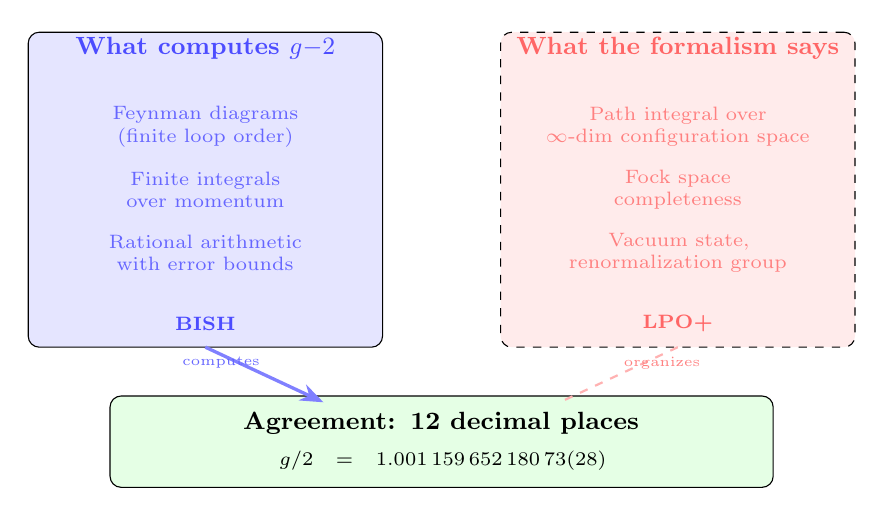
\begin{tikzpicture}[
  >=Stealth,
  every node/.style={font=\small},
  col/.style={draw, rounded corners, minimum width=4.5cm, align=center, inner sep=6pt}
]
% Left column: what actually computes
\node[col, fill=blue!10, minimum height=4cm] (cellar) at (-3, 2) {};
\node[font=\small\bfseries, blue!70] at (-3, 3.8) {What computes $g{-}2$};
\node[font=\scriptsize, blue!60, text width=3.8cm, align=center] at (-3, 2.8)
  {Feynman diagrams\\(finite loop order)};
\node[font=\scriptsize, blue!60, text width=3.8cm, align=center] at (-3, 2.0)
  {Finite integrals\\over momentum};
\node[font=\scriptsize, blue!60, text width=3.8cm, align=center] at (-3, 1.2)
  {Rational arithmetic\\with error bounds};
\node[font=\scriptsize\bfseries, blue!70] at (-3, 0.3) {BISH};

% Right column: the formalism
\node[col, fill=red!8, minimum height=4cm, dashed] (cath) at (3, 2) {};
\node[font=\small\bfseries, red!60] at (3, 3.8) {What the formalism says};
\node[font=\scriptsize, red!50, text width=3.8cm, align=center] at (3, 2.8)
  {Path integral over\\$\infty$-dim configuration space};
\node[font=\scriptsize, red!50, text width=3.8cm, align=center] at (3, 2.0)
  {Fock space\\completeness};
\node[font=\scriptsize, red!50, text width=3.8cm, align=center] at (3, 1.2)
  {Vacuum state,\\renormalization group};
\node[font=\scriptsize\bfseries, red!60] at (3, 0.3) {LPO+};

% Result
\node[draw, rounded corners, fill=green!10, font=\small\bfseries, text width=8cm, align=center, inner sep=6pt]
  (result) at (0, -1.2) {Agreement: 12 decimal places\\[2pt]
  \normalfont\scriptsize $g/2 = 1.001\,159\,652\,180\,73(28)$};

% Arrow from cellar to result
\draw[->, very thick, blue!50] (-3, 0) -- (-1.5, -0.7);
% Disconnected from cathedral
\draw[thick, red!30, dashed] (3, 0) -- (1.5, -0.7);
\node[font=\tiny, red!50] at (2.8, -0.2) {organizes};
\node[font=\tiny, blue!60] at (-2.8, -0.2) {computes};

\end{tikzpicture}
\caption{Act~IV: the most precise prediction in physics.
The $g{-}2$ computation uses finite Feynman diagrams (BISH, solid arrow).
The infinite-dimensional formalism (LPO+, dashed) organizes the computation
but does not contribute to the numerical result.
Twelve decimal places of agreement come from the cellar, not the cathedral.}
\label{fig:g-minus-2}
\end{figure}

% ============================================================
\section{Act~V: The Interpretive Crisis (1975--Present)}
% ============================================================

After the Standard Model was completed in the mid-1970s, the data stream slowed.
The model agreed with every experiment.
New phenomena required higher energies, bigger accelerators, longer timescales, and more money.
Theorists, no longer constrained by a steady flow of surprises from the laboratory, began exploring the mathematical formalism itself.

What they explored was the non-constructive superstructure.

String theory posits a landscape of $10^{500}$ vacuum states---solutions to the equations of the theory that represent possible universes \cite{BoussoPolchinski2000, Susskind2003}.
This is an assertion about the structure of an infinite-dimensional space of solutions.
No finite experiment can probe it.
The many-worlds interpretation of quantum mechanics takes the universal wave function literally, asserting the real physical existence of a branching structure in infinite-dimensional Hilbert space.
No measurement can access the other branches.
The black hole information paradox asks what happens to quantum information at a singularity---combining two LPO-level idealizations (the singularity and the infinite-dimensional state space) into a single problem \cite{AMPS2013}.

From the perspective of the constructive hierarchy, these debates share a structural feature: they are about properties of mathematical objects that live at LPO or higher.
They are questions about the formalism, not about the world.
If you accept that the empirical content of physics is BISH, then a question that can only be \emph{formulated} using LPO or LEM is a question about the mathematical map, not the physical territory.

This diagnosis of the stagnation of theoretical physics is different from, and sharper than, existing critiques.
It does not blame aesthetics, as Hossenfelder does in \emph{Lost in Math}.
It does not blame unfalsifiability, as Woit does in \emph{Not Even Wrong}.
It does not blame sociology, as Smolin does in \emph{The Trouble with Physics}.
It identifies a \emph{structural} correlate: the programmes that have failed to produce testable predictions operate at logical levels that are inherently disconnected from empirical content.
You can explore those levels forever and never produce a prediction that a finite laboratory can test, because the logical distance between the formalism and the predictions is too large.
The formalism is not wrong; it is \emph{idle}---machinery not connected to any output.

A qualification is essential.
Not all post-1975 theoretical work explores the non-constructive superstructure.
Lattice QCD (building on Wilson's 1974 construction \cite{Wilson1974}) has matured into a BISH-level computational programme that predicts hadron masses to percent-level accuracy.
Effective field theory (Weinberg, 1979 onward) organizes finite-order calculations systematically without claiming convergence of the full perturbation series.
Tensor network methods (White 1992, Vidal 2003 onward) provide finite-dimensional variational approaches to quantum many-body systems that avoid infinite-dimensional Hilbert spaces entirely.
Validated numerics and computer-assisted proofs employ interval arithmetic at BISH.
The diagnosis targets specifically those programmes---the string landscape, the multiverse, the information paradox---that operate at logical levels inherently disconnected from finite experiment.
The idle machinery is not ``all post-1975 theory'' but the subset that explores the non-constructive superstructure without producing BISH-level predictions.

\begin{figure}[ht]
\centering
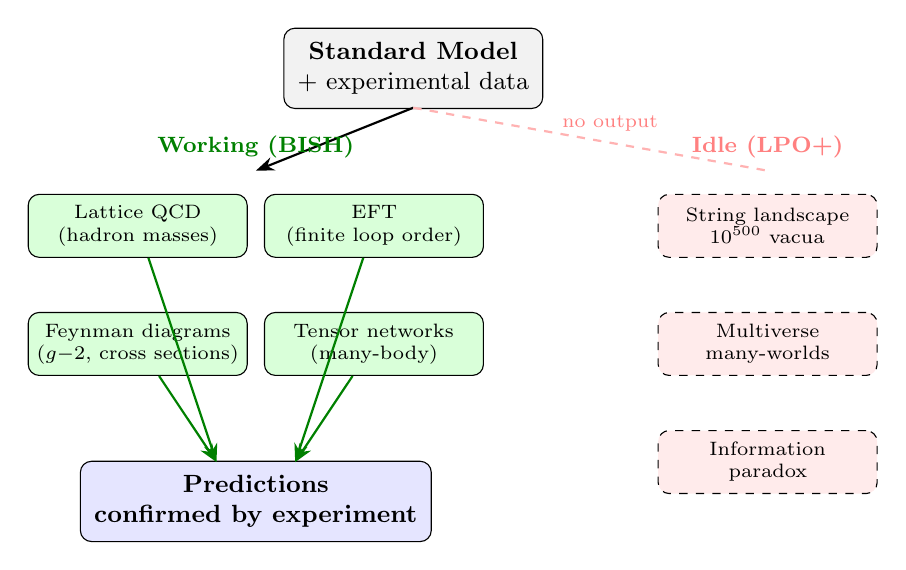
\begin{tikzpicture}[
  >=Stealth,
  every node/.style={font=\small},
  gear/.style={draw, rounded corners, minimum height=0.8cm, align=center, inner sep=4pt, font=\scriptsize}
]
% Input
\node[draw, rounded corners, fill=gray!10, minimum width=3cm, align=center, inner sep=5pt]
  (input) at (0, 3.5) {\textbf{Standard Model}\\+ experimental data};

% Working machinery (BISH)
\node[gear, fill=green!15, text width=2.5cm] (lqcd) at (-3.5, 1.5) {Lattice QCD\\(hadron masses)};
\node[gear, fill=green!15, text width=2.5cm] (eft) at (-0.5, 1.5) {EFT\\(finite loop order)};
\node[gear, fill=green!15, text width=2.5cm] (feyn) at (-3.5, 0) {Feynman diagrams\\($g{-}2$, cross sections)};
\node[gear, fill=green!15, text width=2.5cm] (tensor) at (-0.5, 0) {Tensor networks\\(many-body)};

% Idle machinery (LPO+)
\node[gear, fill=red!8, dashed, text width=2.5cm] (string) at (4.5, 1.5) {String landscape\\$10^{500}$ vacua};
\node[gear, fill=red!8, dashed, text width=2.5cm] (multi) at (4.5, 0) {Multiverse\\many-worlds};
\node[gear, fill=red!8, dashed, text width=2.5cm] (info) at (4.5, -1.5) {Information\\paradox};

% Output
\node[draw, rounded corners, fill=blue!10, minimum width=3cm, align=center, inner sep=5pt, font=\small\bfseries]
  (output) at (-2, -2) {Predictions\\confirmed by experiment};

% Arrows
\draw[->, thick] (0, 3.0) -- (-2, 2.2);
\draw[->, thick, green!50!black] (lqcd) -- (-2.5, -1.5);
\draw[->, thick, green!50!black] (eft) -- (-1.5, -1.5);
\draw[->, thick, green!50!black] (feyn) -- (-2.5, -1.5);
\draw[->, thick, green!50!black] (tensor) -- (-1.5, -1.5);

% No connection from idle
\draw[thick, red!30, dashed] (0, 3.0) -- (4.5, 2.2);
\node[font=\scriptsize, red!50] at (2.5, 2.8) {no output};

% Labels
\node[font=\footnotesize\bfseries, green!50!black] at (-2, 2.5) {Working (BISH)};
\node[font=\footnotesize\bfseries, red!50] at (4.5, 2.5) {Idle (LPO+)};

\end{tikzpicture}
\caption{Act~V: working machinery vs.\ idle machinery.
Post-1975 physics divides into programmes that produce BISH-level predictions confirmed by experiment
(left, green) and programmes that explore the non-constructive superstructure without
empirical output (right, red/dashed).
The diagnosis is structural: the idle machinery operates at logical levels disconnected from finite experiment.}
\label{fig:idle-machinery}
\end{figure}

The constructive hierarchy suggests a diagnosis and a remedy: the next breakthrough may require \emph{less} logical structure, not more---the identification of which parts of the existing formalism are physically idle and their careful removal.

\textbf{The constructive alternative.}
Bishop's \emph{Foundations of Constructive Analysis} (1967) \cite{Bishop1967} proved that the core of mathematical analysis survives constructively; his 1973 lectures diagnosed contemporary mathematics as suffering from a ``schizophrenia'' between formal manipulation and computational meaning.
Since 2019, Nicolas Gisin---a physicist with Nobel-adjacent credentials in quantum nonlocality---has argued that real numbers are ``the hidden variables of classical physics,'' that intuitionistic mathematics is the natural language for finite physical systems, and that the apparent determinism of classical mechanics is an artifact of using real numbers with infinite information content \cite{Gisin2020, Gisin2021}.
Gisin provides the philosophical vision; our programme supplies the formal precision his broad-brush argument lacks (see Section~\ref{sec:thesis}).

\begin{keymessage}
Post-Standard-Model theoretical physics explores logical levels disconnected from experiment.
The diagnosis is structural: formalism at LPO+ cannot produce BISH-level predictions.
Working programmes (lattice QCD, EFT, tensor networks) remain at BISH\@.
The idle machinery is not all post-1975 theory---only the subset that explores the non-constructive superstructure.
\end{keymessage}


% ============================================================
\section{The Logical Geography: What the Proofs Show}
% ============================================================

The preceding narrative rests on a specific body of evidence: a calibration table mapping layers of mathematical physics to their precise position in the constructive hierarchy.
Each entry is machine-verified in the Lean~4 proof assistant, using either constructive reverse mathematics (CRM) over the Mathlib library \cite{Ishihara2006, BridgesVita2006} or an axiom-calibration framework in standalone Lean.

\begin{figure}[ht]
\centering
\resizebox{0.92\textwidth}{!}{%
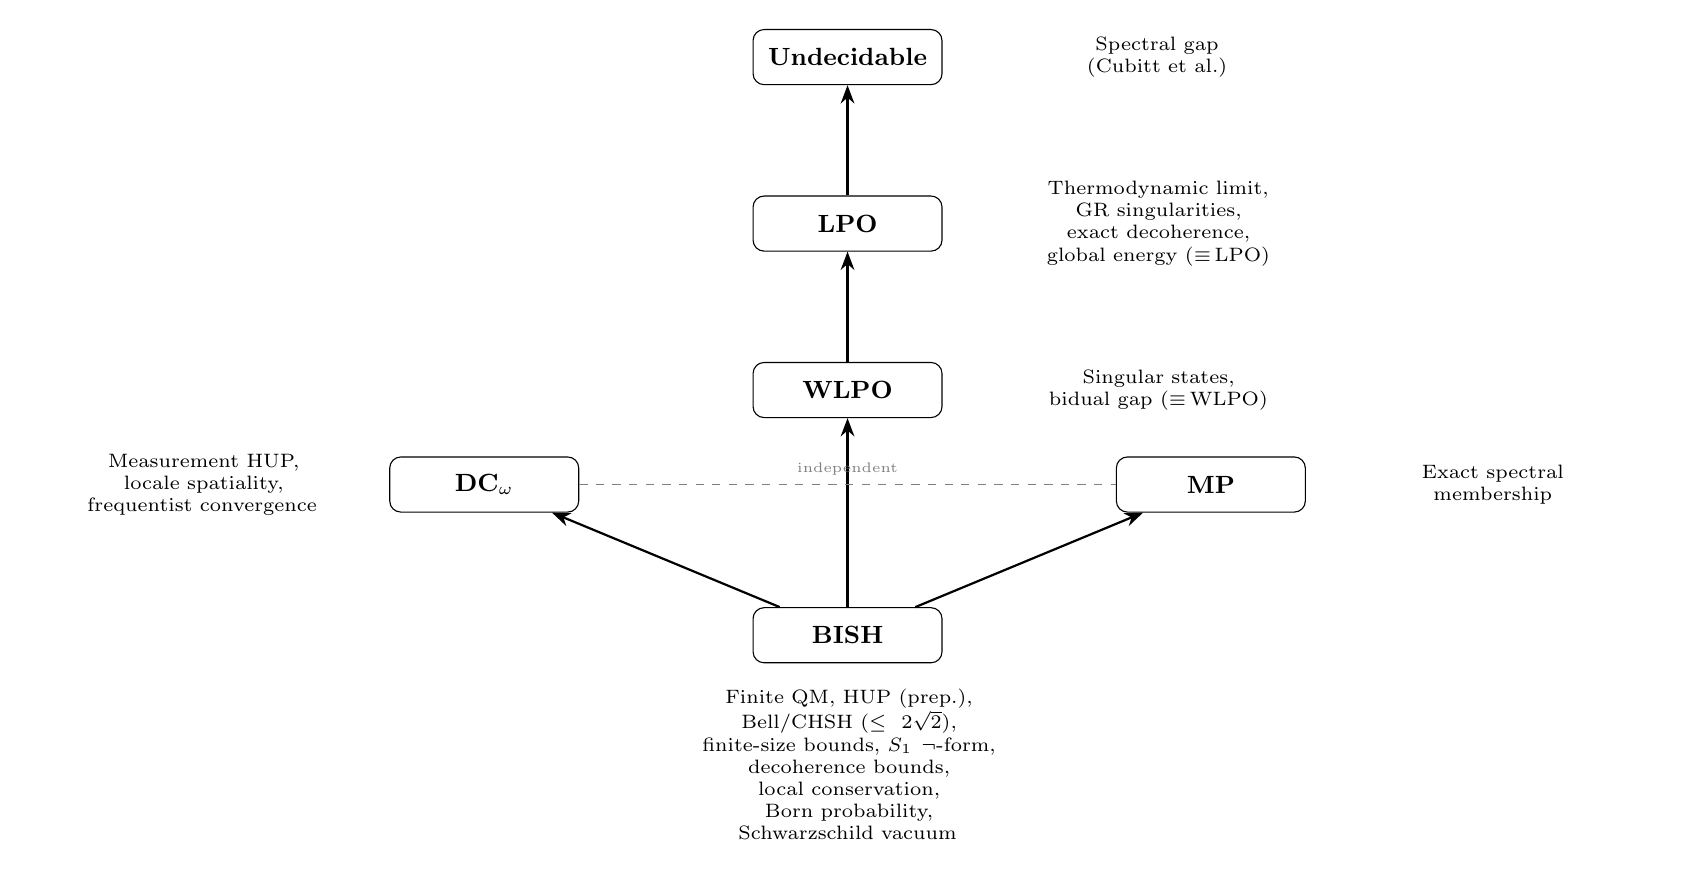
\begin{tikzpicture}[
  node distance=1.4cm and 2.8cm,
  principle/.style={draw, rounded corners, minimum width=2.4cm, minimum height=0.7cm, font=\small\bfseries},
  physlabel/.style={font=\scriptsize, text width=4.2cm, align=center},
  >=Stealth
]
% Main spine
\node[principle] (bish) {BISH};
\node[principle, above=2.4cm of bish] (wlpo) {WLPO};
\node[principle, above=of wlpo] (lpo) {LPO};
\node[principle, above=of lpo] (undec) {Undecidable};

% Orthogonal branches
\node[principle, above left=1.2cm and 2.2cm of bish] (dc) {DC$_\omega$};
\node[principle, above right=1.2cm and 2.2cm of bish] (mp) {MP};

% Edges (Hasse diagram: only covering relations)
\draw[thick, ->] (bish) -- (dc);
\draw[thick, ->] (bish) -- (mp);
\draw[thick, ->] (bish) -- (wlpo);
\draw[thick, ->] (wlpo) -- (lpo);
\draw[thick, ->] (lpo) -- (undec);

% Physical labels
\node[physlabel, below=0.2cm of bish] {Finite QM, HUP (prep.),\\Bell/CHSH ($\leq 2\sqrt{2}$),\\finite-size bounds, $S_1\;\neg$-form,\\decoherence bounds, local conservation,\\Born probability, Schwarzschild vacuum};
\node[physlabel, left=0.15cm of dc] {Measurement HUP,\\locale spatiality,\\frequentist convergence};
\node[physlabel, right=0.15cm of mp] {Exact spectral\\membership};
\node[physlabel, right=0.5cm of wlpo] {Singular states,\\bidual gap ($\equiv$\,WLPO)};
\node[physlabel, right=0.5cm of lpo] {Thermodynamic limit,\\GR singularities,\\exact decoherence,\\global energy ($\equiv$\,LPO)};
\node[physlabel, right=0.5cm of undec] {Spectral gap\\(Cubitt et al.)};

% Orthogonality annotation
\draw[dashed, gray] (dc) -- node[above, font=\tiny, gray] {independent} (mp);

\end{tikzpicture}%
}% end resizebox
\caption{The logical geography of mathematical physics: a Hasse diagram.
Arrows indicate strict implication over BISH. The omniscience spine
(BISH $<$ WLPO $<$ LPO) forms the dominant vertical chain. DC$_\omega$ and MP
occupy orthogonal positions: neither implies the other, and neither implies WLPO.
Physical layers are annotated with their calibrated logical cost.
All entries are machine-verified; ``$\equiv$'' denotes proven equivalence over BISH.}
\label{fig:hasse}
\end{figure}

The calibration table is displayed in Figure~\ref{fig:hasse}.
Return to the mountain metaphor.

\textbf{Sea level (BISH).}
Everything a laboratory does lives here.
Finite quantum mechanics: unitary evolution, Born rule probabilities, measurements on finite-dimensional systems.
Preparation uncertainty: the Robertson-Schr\"odinger inequality~\eqref{eq:rs-inequality}, a pure Cauchy-Schwarz argument.
Bell nonlocality: the Tsirelson bound~\eqref{eq:chsh} on CHSH correlations.
Entanglement entropy of qubit systems: the Bell singlet partial trace yields $\operatorname{Tr}_B(|\Psi^-\rangle\langle\Psi^-|) = \tfrac{1}{2}I_2$, giving maximal entanglement entropy $h(1/2) = \log 2$---all explicit matrix arithmetic, BISH.
Finite-size error bounds~\eqref{eq:ising-bound} for the one-dimensional Ising model.
Local general relativity: the Raychaudhuri focusing equation~\eqref{eq:raychaudhuri}, the Schwarzschild vacuum solution with its constructively computable Kretschmann invariant $K = 48M^2/r^6$.
Decoherence bounds: the off-diagonal decay estimate $|\rho_{01}(t)| \leq e^{-\gamma t}$ for a qubit coupled to an $N$-mode environment, pure finite-dimensional linear algebra (Paper~14) \cite{Lee2026j}.
Local conservation laws: Noether currents and continuity equations for finite lattice systems, including local energy-momentum conservation on finite grids (Paper~15) \cite{Lee2026k}.
Born-rule probabilities: the derivation of $p_k = |\langle \phi_k | \psi \rangle|^2$ from the projection postulate via finite-dimensional inner products (Paper~16) \cite{Lee2026l}.
All of these are provable without any omniscience principle or appeal to the law of excluded middle.

\textbf{The foothills (Dependent Choice, Markov's Principle).}
Measurement uncertainty---extracting classical statistics from an infinite sequence of quantum measurements---requires Dependent Choice \cite{Lee2026g}.
Exact spectral membership---asserting that a specific value belongs to the spectrum of an operator---requires Markov's Principle \cite{Lee2026f}.
Frequentist convergence---the assertion that Born-rule probabilities emerge as limiting relative frequencies over an infinite sequence of identical measurements---requires DC$_\omega$ for the sequential construction of the frequency limit \cite{Lee2026l}.
These principles are independent of each other and independent of WLPO.
The logical geography is not a simple linear chain; it has lateral dimensions.

\textbf{The mountainside (WLPO).}
Singular states---functionals in the bidual of the trace-class operators that correspond to no density matrix---require WLPO to construct \cite{Lee2026a, Lee2026b}.
The bidual gap, the separation between physical states and mathematical artifacts of the infinite-dimensional formalism, costs exactly WLPO.

\textbf{The summit (LPO).}
The thermodynamic limit: the assertion that the free energy per particle converges to a definite real number as the system size grows without bound.
This is equivalent to LPO over constructive mathematics---proved for the one-dimensional Ising model \cite{Lee2026c} and verified across two independent mathematical formulations (transfer-matrix and combinatorial \cite{Lee2026e}), establishing that the logical cost is intrinsic to the physics, not an artifact of the proof technique.
The same BMC~$\equiv$~LPO equivalence governs geodesic incompleteness in general relativity \cite{Lee2026paper13}: the completed-limit assertion that every bounded monotone trajectory in the Schwarzschild interior converges.
The same BMC~$\equiv$~LPO equivalence governs two further domains: exact decoherence in open quantum systems---the assertion that off-diagonal density matrix elements converge to zero as the environment grows (Paper~14) \cite{Lee2026j}---and global energy conservation---the assertion that Noether-conserved quantities persist through infinitely many time steps (Paper~15) \cite{Lee2026k}.
This \emph{domain invariance}---the same logical cost appearing in statistical mechanics, gravitation, quantum decoherence, and conservation laws through the same abstract principle---strengthens the evidence that the costs are intrinsic to the operation of passing from a bounded monotone sequence to its limit, regardless of the physical domain that produces the sequence.

\textbf{Beyond the summit (undecidable).}
The spectral gap problem---whether the Hamiltonian of an infinite lattice system has a gap above the ground state energy---is undecidable in the sense of Turing: no algorithm can determine the answer from the Hamiltonian's local interaction rules \cite{Cubitt2015}.
This is not ``a level above LEM'' in the logical hierarchy; it is an orthogonal phenomenon.
LEM does not help you compute an uncomputable function.
Undecidability means that the idealization strategy hits a different kind of ceiling---not insufficient logical strength, but the inherent limitation of algorithmic procedures applied to infinite lattice systems.
The summit of the omniscience hierarchy (LPO) and Turing undecidability are distinct obstructions, and conflating them would misrepresent both.

Yet the two hierarchies share a common boundary.
For any \emph{finite} lattice, the spectral gap is a computable real number---eigenvalues of a finite Hermitian matrix are BISH, and the question ``is the gap above~$\varepsilon$?'' is decidable by rational approximation.
The undecidability of Cubitt et~al.\ enters only through the thermodynamic limit $N \to \infty$---the same limit that costs LPO in the Ising calibration.
The constructive hierarchy and the computability hierarchy are orthogonal axes, but they agree on where the physics--formalism boundary falls: finite systems sit at BISH/decidable, and infinite idealizations sit above BISH in both.
A similar pattern appears in the foundations of quantum correlations.
The set of correlations achievable by finite-dimensional quantum systems is identical whether formalized via tensor products or commuting operators, and the Tsirelson bound $2\sqrt{2}$ holds in both formalizations at BISH \cite{Lee2026paper11}.
Ji, Natarajan, Vidick, Wright, and Yuen showed that this equivalence fails catastrophically in infinite dimensions: the membership problem for infinite-dimensional commuting-operator correlations is RE-complete---as hard as the halting problem \cite{JNVWY2021}.
The physical correlations, preparable with finite entanglement and measurable by finite apparatus, are BISH and formalization-invariant.
The mathematical excess---correlations requiring infinite entanglement in infinite-dimensional spaces---is where the formalizations diverge, and the divergence reaches the highest levels of the computability hierarchy.
Neither result has been calibrated against the omniscience hierarchy (that would require proving specific equivalences with WLPO, LPO, or higher principles, which remains open), but both confirm the programme's central pattern: physical content at BISH, with logical cost increasing monotonically as the formalism extends beyond the finite.

\begin{figure}[ht]
\centering
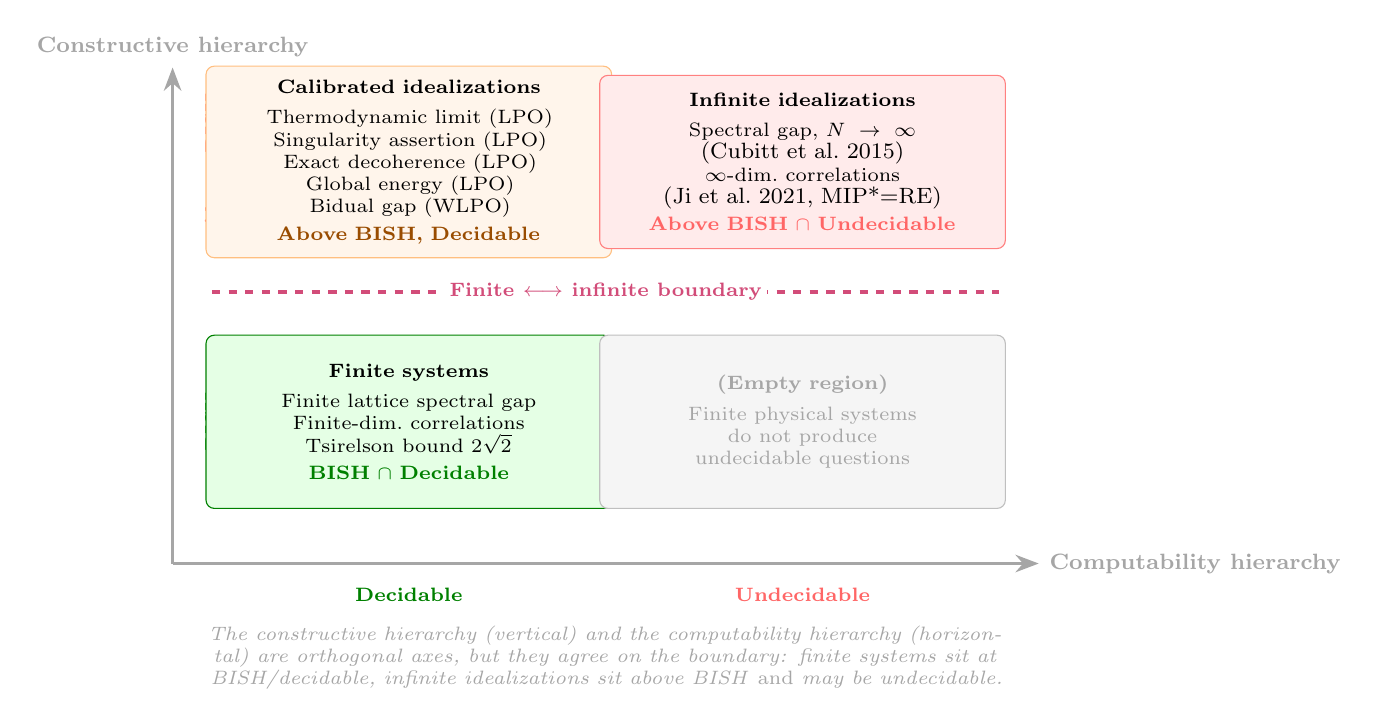
\begin{tikzpicture}[
  >=Stealth,
  every node/.style={font=\small},
  cell/.style={draw, rounded corners=3pt, font=\scriptsize,
               minimum height=2.2cm, text width=4.8cm, align=center,
               inner sep=5pt}
]
% ---- Axes ----
\draw[->, very thick, gray!70] (-5.5, -1.8) -- (-5.5, 4.5)
  node[above, font=\footnotesize\bfseries, gray!70] {Constructive hierarchy};
\draw[->, very thick, gray!70] (-5.5, -1.8) -- (5.5, -1.8)
  node[right, font=\footnotesize\bfseries, gray!70] {Computability hierarchy};

% ---- Axis labels ----
\node[font=\scriptsize\bfseries, green!50!black, rotate=90] at (-5.0, 0) {BISH};
\node[font=\scriptsize\bfseries, red!60, rotate=90] at (-5.0, 3.3) {Above BISH};
\node[font=\scriptsize\bfseries, green!50!black] at (-2.5, -2.2) {Decidable};
\node[font=\scriptsize\bfseries, red!60] at (2.5, -2.2) {Undecidable};

% ---- Bottom-left: BISH + Decidable ----
\node[cell, fill=green!10, draw=green!50!black] at (-2.5, 0)
  {\textbf{Finite systems}\\[3pt]
   Finite lattice spectral gap\\
   Finite-dim.\ correlations\\
   Tsirelson bound $2\sqrt{2}$\\[2pt]
   \textcolor{green!50!black}{\textbf{BISH $\cap$ Decidable}}};

% ---- Top-left: Above BISH + Decidable ----
\node[cell, fill=orange!8, draw=orange!50] at (-2.5, 3.3)
  {\textbf{Calibrated idealizations}\\[3pt]
   Thermodynamic limit (LPO)\\
   Singularity assertion (LPO)\\
   Exact decoherence (LPO)\\
   Global energy (LPO)\\
   Bidual gap (WLPO)\\[2pt]
   \textcolor{orange!60!black}{\textbf{Above BISH, Decidable}}};

% ---- Top-right: Above BISH + Undecidable ----
\node[cell, fill=red!8, draw=red!50] at (2.5, 3.3)
  {\textbf{Infinite idealizations}\\[3pt]
   Spectral gap, $N\!\to\!\infty$\\
   {\footnotesize (Cubitt et al.\ 2015)}\\
   $\infty$-dim.\ correlations\\
   {\footnotesize (Ji et al.\ 2021, MIP*=RE)}\\[2pt]
   \textcolor{red!60}{\textbf{Above BISH $\cap$ Undecidable}}};

% ---- Bottom-right: BISH + Undecidable (empty/impossible) ----
\node[cell, fill=gray!8, draw=gray!50, text=gray!70] at (2.5, 0)
  {\textbf{(Empty region)}\\[3pt]
   Finite physical systems\\
   do not produce\\
   undecidable questions};

% ---- Diagonal pattern ----
\draw[very thick, dashed, purple!70] (-5.0, 1.65) -- (5.0, 1.65);
\node[font=\scriptsize\bfseries, purple!70, fill=white, inner sep=2pt]
  at (0, 1.65) {Finite $\longleftrightarrow$ infinite boundary};

% ---- Key annotation ----
\node[font=\scriptsize\itshape, gray!70, text width=10cm, align=center]
  at (0, -3.0)
  {The constructive hierarchy (vertical) and the computability hierarchy (horizontal)
   are orthogonal axes, but they agree on the boundary: finite systems sit at
   BISH/decidable, infinite idealizations sit above BISH \emph{and} may be undecidable.};

\end{tikzpicture}
\caption{Two orthogonal hierarchies, one boundary.
The constructive hierarchy (omniscience principles) and the computability hierarchy
(decidability/Turing degrees) are logically independent axes.
Yet they agree on where the physics--formalism boundary falls:
finite systems are BISH and decidable; infinite idealizations are above BISH in both.
The Cubitt et~al.\ spectral gap undecidability and the Ji et~al.\ MIP*\,=\,RE result
both enter through the same $N \to \infty$ passage that costs LPO in the Ising calibration.
Neither result has been calibrated against the omniscience hierarchy (dashed lines indicate open questions).}
\label{fig:undecidability}
\end{figure}

Two features of this table deserve emphasis.

First, \emph{formulation-invariance}.
The LPO cost of the thermodynamic limit was derived independently via two completely different mathematical routes: a transfer-matrix method using eigenvalue analysis and linear algebra, and a purely combinatorial method using bond variables and a binomial parity sieve with no matrices or functional analysis \cite{Lee2026e}.
The axiom profiles are identical.
This is evidence that the logical cost is a property of the physics, not of the mathematician's choice of formalism.

Second, \emph{machine verification}.
These results are not informal arguments about what ``should'' be constructive.
They are Lean~4 proof terms, machine-checked end-to-end, with \texttt{\#print axioms} certificates that list every non-constructive axiom used in each proof.
The total is approximately 12,000~lines of formally verified code.
The proof assistant enforces the logical bookkeeping that human mathematicians cannot reliably perform: it ensures that no classical axiom sneaks in through a library import, a typeclass resolution, or an unnoticed appeal to decidability.

\begin{keymessage}
The calibration table maps physics to exact logical levels, machine-verified in ${\sim}12{,}000$ lines of Lean~4.
Key findings: \emph{formulation-invariance} (same cost via different proofs) and \emph{domain invariance} (same cost across four independent physical domains) show the logical costs are intrinsic, not artifacts of the formalism.
\end{keymessage}

% ============================================================
\section{What Could Have Been Done Instead}
\label{sec:alternatives}
% ============================================================

The calibration table is not merely a diagnosis; it suggests a therapy.
The remarkable fact is that physicists \emph{already compute at BISH}---they just don't know it.
The constructive alternatives to the classical formalism are not radical proposals for a new physics.
They are descriptions of what physicists actually do: finite-size error bounds instead of the thermodynamic limit~\eqref{eq:ising-bound}, the Cauchy-Schwarz inequality instead of spectral theory for uncertainty~\eqref{eq:rs-inequality}, finite-dimensional linear algebra for Bell nonlocality~\eqref{eq:chsh}, finite-parameter differential equations for gravitational focusing~\eqref{eq:raychaudhuri}, and finite-order Feynman diagrams instead of path integrals.
In every case the constructive alternative is what the working physicist is already doing.
The formalism merely pretends otherwise.

Moreover, several post-war developments in mathematical physics are themselves constructive frameworks, often unrecognized as such:
\begin{itemize}[nosep]
\item \textbf{Wilson's lattice gauge theory (1974) \cite{Wilson1974}}: a rigorous,
  finite-dimensional framework for non-perturbative QFT\@. Lattice QCD computes
  hadron masses, the proton charge radius, and quark masses from first
  principles---all on finite grids with controlled errors. This is BISH\@.
\item \textbf{Effective field theory} (Weinberg, 1979+): a systematic
  organizing principle that keeps calculations at finite loop order without
  claiming convergence of the full perturbation series.
\item \textbf{Tensor network methods} (White 1992, Vidal 2003+):
  finite-dimensional variational approaches to quantum many-body systems
  (DMRG, MERA, PEPS) that avoid infinite-dimensional Hilbert spaces entirely.
\item \textbf{Validated numerics}: interval arithmetic and computer-assisted
  proofs that produce rigorous finite-precision bounds---constructive
  mathematics in practice.
\end{itemize}
The constructive alternative is not a hypothetical programme; it is how much of contemporary computational physics already operates.

\begin{figure}[ht]
\centering
\resizebox{\textwidth}{!}{%
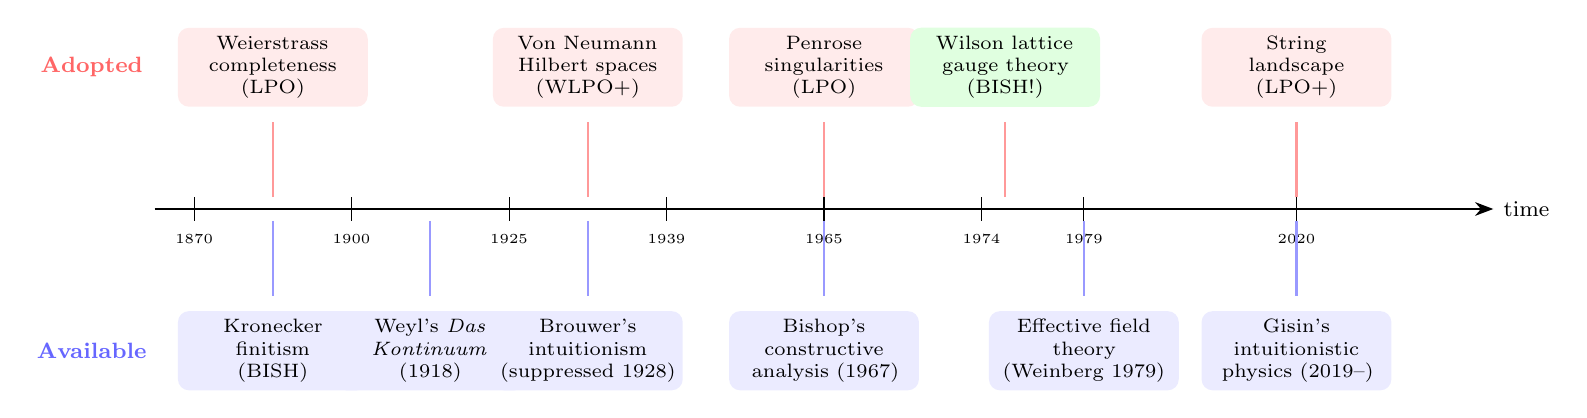
\begin{tikzpicture}[
  >=Stealth,
  every node/.style={font=\scriptsize},
  event/.style={circle, fill, inner sep=1.5pt},
  adopted/.style={font=\scriptsize, text width=2.2cm, align=center, fill=red!8, rounded corners, inner sep=3pt},
  alternative/.style={font=\scriptsize, text width=2.2cm, align=center, fill=blue!8, rounded corners, inner sep=3pt}
]
% Timeline
\draw[thick, ->] (0,0) -- (17, 0) node[right] {\footnotesize time};
% Tick marks
\foreach \x/\y in {0.5/1870, 2.5/1900, 4.5/1925, 6.5/1939, 8.5/1965, 10.5/1974, 11.8/1979, 14.5/2020} {
  \draw (\x, -0.15) -- (\x, 0.15);
  \node[below, font=\tiny] at (\x, -0.2) {\y};
}
% Upper track: what was adopted (red-tinted)
\node[adopted] at (1.5, 1.8) {Weierstrass\\completeness\\(LPO)};
\node[adopted] at (5.5, 1.8) {Von Neumann\\Hilbert spaces\\(WLPO+)};
\node[adopted] at (8.5, 1.8) {Penrose\\singularities\\(LPO)};
\node[adopted, fill=green!12] at (10.8, 1.8) {Wilson lattice\\gauge theory\\(BISH!)};
\node[adopted] at (14.5, 1.8) {String\\landscape\\(LPO+)};
% Lower track: what was available (blue-tinted)
\node[alternative] at (1.5, -1.8) {Kronecker\\finitism\\(BISH)};
\node[alternative] at (3.5, -1.8) {Weyl's \emph{Das\\Kontinuum}\\(1918)};
\node[alternative] at (5.5, -1.8) {Brouwer's\\intuitionism\\(suppressed 1928)};
\node[alternative] at (8.5, -1.8) {Bishop's\\constructive\\analysis (1967)};
\node[alternative] at (11.8, -1.8) {Effective field\\theory\\(Weinberg 1979)};
\node[alternative] at (14.5, -1.8) {Gisin's\\intuitionistic\\physics (2019--)};
% Arrows connecting to timeline
\foreach \x in {1.5, 5.5, 8.5, 10.8, 14.5} {
  \draw[red!40, thick] (\x, 0.15) -- (\x, 1.1);
}
\foreach \x in {1.5, 3.5, 5.5, 8.5, 11.8, 14.5} {
  \draw[blue!40, thick] (\x, -0.15) -- (\x, -1.1);
}
% Labels for tracks
\node[font=\footnotesize\bfseries, red!60] at (-0.8, 1.8) {Adopted};
\node[font=\footnotesize\bfseries, blue!60] at (-0.8, -1.8) {Available};
\end{tikzpicture}%
}% end resizebox
\caption{The road not taken. At every stage where classical logic was imported into
physics (upper track, red), a constructive alternative was available (lower track, blue).
Wilson's lattice gauge theory (green, 1974) is the exception: an adopted framework
that is itself BISH\@.
The constructive road was not taken---not because it was mathematically inadequate,
but because the classical road was more convenient and its logical cost was invisible.}
\label{fig:timeline}
\end{figure}

\begin{keymessage}
At every stage, constructive alternatives existed (Figure~\ref{fig:timeline}).
Lattice QCD, effective field theory, tensor networks, and validated numerics are already BISH frameworks.
The constructive alternative is not a hypothetical programme---it is what physicists already do.
\end{keymessage}

\subsection*{The cognitive value of idealization}

If the constructive alternative suffices for every prediction, a natural objection arises: why did every great physicist of the twentieth century use the cathedral?
Einstein was not confused.
Von~Neumann was not following convention.
Dirac was not ignorant of alternatives.
They chose the idealizations because the idealizations let them \emph{think}.

Consider the path to general relativity.
Einstein's 1915 field equations $G_{\mu\nu} = 8\pi T_{\mu\nu}$ are a finite system of PDEs relating finite objects---metric components, their derivatives, stress-energy.
Writing them down requires no idealization; the route to them through differential geometry and tensor calculus is algebraic and BISH\@.
But Einstein arrived at these equations by thinking of spacetime as a smooth manifold, gravity as curvature, geodesics as paths of free particles.
That geometric picture, while not formally requiring non-constructive logic, is deeply entangled with the idea of a completed continuum---a smooth, infinite, everywhere-defined mathematical object.
The picture guided ten years of creative struggle (1905--1915).

Once the equations were written, every empirical prediction Einstein extracted was BISH\@.
The perihelion precession of Mercury: a perturbative solution of the geodesic equation in the Schwarzschild metric, yielding $\delta\varphi = 6\pi GM/(c^2 a(1-e^2))$.
Finite computation, algebraic result.
Gravitational redshift: $\nu_2/\nu_1 = \sqrt{g_{00}(r_1)/g_{00}(r_2)}$.
One formula, one substitution.
Gravitational lensing: $\delta = 4GM/(c^2 b)$.
A definite integral with an explicit integrand.
Every number Einstein compared with observation was a BISH computation from specific equations evaluated at specific parameters.

The same pattern holds for quantum mechanics.
Heisenberg's 1925 matrix mechanics was explicitly finite and algebraic---transition amplitudes as finite matrix elements, the hydrogen spectrum by finite matrix truncation.
This is BISH\@.
Schr\"odinger's 1926 wave mechanics introduced the wave function $\psi(x) \in L^2(\mathbb{R}^3)$---an infinite-dimensional Hilbert space---but every calculation Schr\"odinger actually performed reduced to solving a specific differential equation with specific boundary conditions.
The hydrogen eigenvalue $E_n = -13.6/n^2$~eV comes from a boundary-value problem for a second-order ODE; each specific eigenvalue is computable by algebraic manipulation.
No spectral theorem is invoked.
The spectral theorem enters when you assert that these are \emph{all} the eigenvalues and that the eigenfunctions form a \emph{complete} basis---an assertion about a completed infinite object that organizes the physics but generates no additional predictions.

The idealizations serve as \emph{cognitive infrastructure}: they convert processes into objects.
The thermodynamic limit converts an open-ended approximation (``the free energy per site is within~$\varepsilon$ of $f(\beta)$ for lattice size $N(\varepsilon)$'') into a definite fact (``the free energy is $f(\beta)$'').
The first is a bound you can compute with.
The second is a thought you can compose with other thoughts---you can differentiate it, take its Legendre transform, study its singularities.
The spectral theorem converts an open-ended list (``these specific eigenvalues satisfy these specific equations'') into a completed structure (``every self-adjoint operator has a spectral decomposition'').
The first handles specific systems.
The second enables general theory---perturbation theory, scattering theory, the classification of quantum symmetries.
Each idealization converts a BISH computation into a mathematical object that can be manipulated, composed, and reasoned about at a higher level of abstraction.
The logical cost, measured by the calibration table, is the price of that conversion.

This reinterpretation answers the essential-idealizations objection directly.
Batterman~\cite{Batterman2005} argues that infinite idealizations are ``explanatorily essential''---that the thermodynamic limit genuinely explains universality in a way finite-system descriptions do not.
We can now agree partially: the idealization is \emph{cognitively} essential, in the sense that it enables reasoning, explanation, and theory-building that the finite descriptions cannot support at comparable cognitive cost.
But it is not \emph{computationally} essential: every number the explanation predicts is extractable from the BISH cellar.
The cathedral is not a computing device.
It is a thinking device.
Its value is real.
Its logical cost is measurable.
Its computational content is zero.
Conversely, when a formalism's non-constructive infrastructure generates assertions beyond BISH---the termination of spacetime at a singularity, the preparation of a singular quantum state---the calibration table identifies these not as predictions awaiting experimental confirmation but as artefacts of the idealization, statements the mathematics makes but no finite experiment can adjudicate.
The calibration table thus serves as both asset ledger and hazard register: it records the cognitive value each idealization purchases and flags the pseudo-predictions it generates as a byproduct.

The calibration table suggests a criterion for distinguishing safe from potentially pathological idealizations.
An idealization is safe when it serves as a shortcut: non-constructive reasoning is introduced at one level of the hierarchy, but every downstream prediction can be independently extracted at BISH\@.
The thermodynamic limit exemplifies this pattern---the passage to infinite~$N$ lives at LPO, but every observable consequence (phase transition temperatures, critical exponents) is recoverable from finite-$N$ computations with explicit error bounds.
The idealization becomes \emph{potentially} pathological when its non-constructive output propagates downstream and is treated as physical input to further reasoning---though one cannot rule out that nature itself enforces the idealization.
The Schwarzschild singularity illustrates the concern: geodesic incompleteness is an LPO-level assertion about manifold completeness, yet the black hole information paradox feeds it into quantum-mechanical arguments as a physical boundary condition---as if spacetime termination were an empirical fact rather than an artefact of the completed limit.
The calibration table makes this diagnostic mechanical: trace the logical level of each assertion through the derivation chain, and flag any point where content above BISH enters subsequent reasoning as if it were a physical datum.

\begin{figure}[H]
\centering
\resizebox{\textwidth}{!}{%
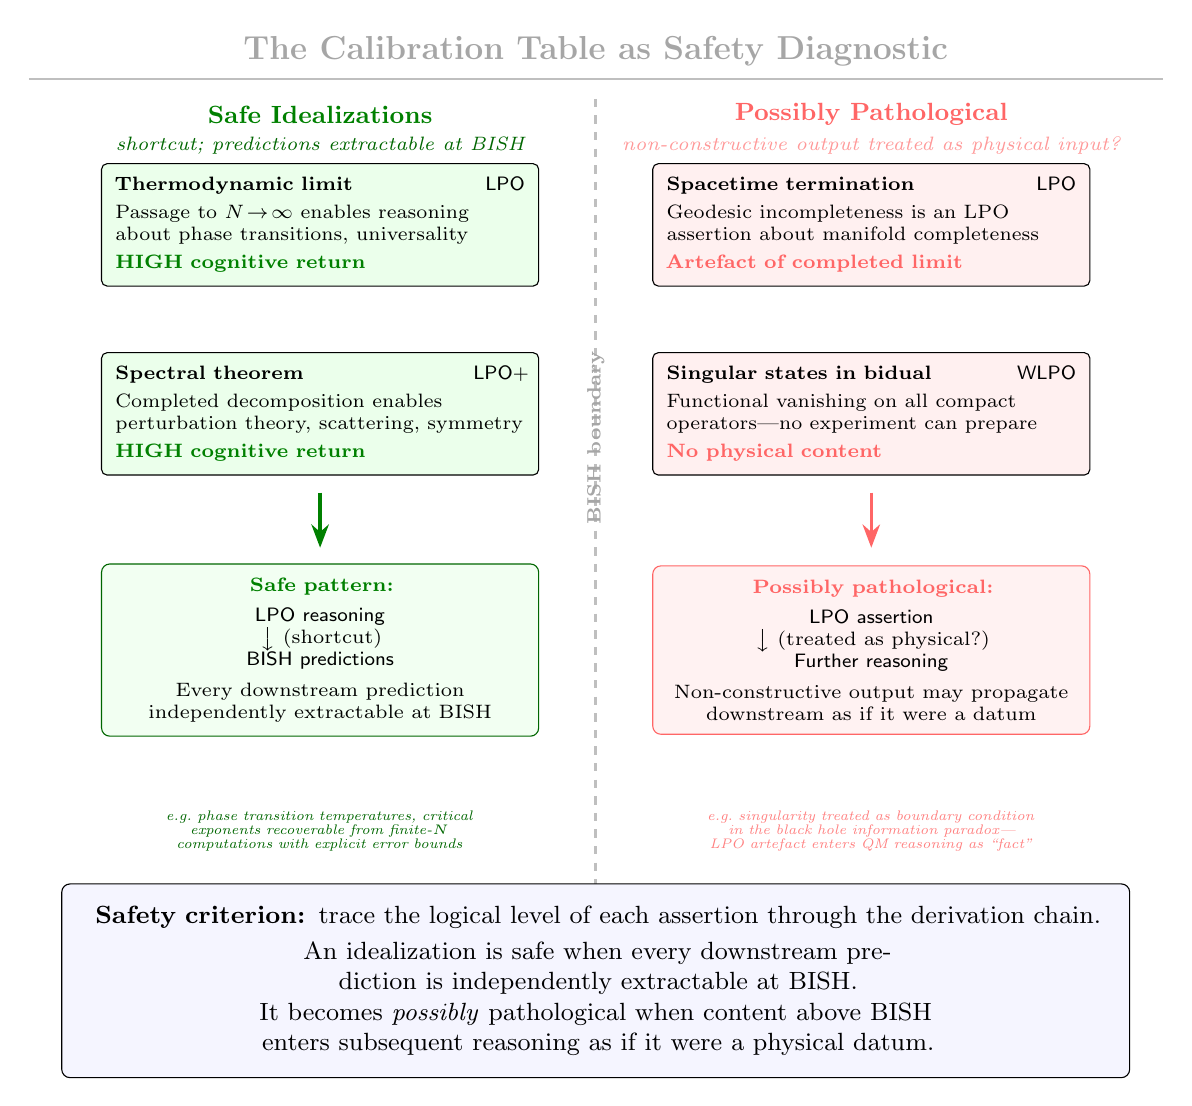
\begin{tikzpicture}[
  >=Stealth,
  every node/.style={font=\small},
  entry/.style={draw, rounded corners=2pt, font=\scriptsize,
                text width=5.2cm, align=left, inner sep=5pt},
  flowbox/.style={draw, rounded corners=3pt, font=\scriptsize,
                  text width=5.2cm, align=center, inner sep=5pt}
]
% ---- HEADER ----
\node[font=\large\bfseries, gray!70] at (0, 9.4)
  {The Calibration Table as Safety Diagnostic};
\draw[thick, gray!50] (-7.2, 9.05) -- (7.2, 9.05);

% ==== LEFT: Safe Idealizations ====
\node[font=\small\bfseries, green!50!black] at (-3.5, 8.6)
  {Safe Idealizations};
\node[font=\scriptsize\itshape, green!40!black] at (-3.5, 8.2)
  {shortcut; predictions extractable at BISH};

\node[entry, fill=green!8] (thermo) at (-3.5, 7.2) {%
  \textbf{Thermodynamic limit} \hfill\textsf{LPO}\\[2pt]
  Passage to $N\!\to\!\infty$ enables reasoning\\
  about phase transitions, universality\\[2pt]
  \textbf{\color{green!50!black}HIGH cognitive return}};

\node[entry, fill=green!8] (spectral) at (-3.5, 4.8) {%
  \textbf{Spectral theorem} \hfill\textsf{LPO+}\\[2pt]
  Completed decomposition enables\\
  perturbation theory, scattering, symmetry\\[2pt]
  \textbf{\color{green!50!black}HIGH cognitive return}};

% ---- Left flow: SAFE pattern ----
\draw[->, very thick, green!50!black]
  (-3.5, 3.8) -- (-3.5, 3.1);

\node[flowbox, fill=green!5, draw=green!40!black] (safeflow)
  at (-3.5, 1.8) {%
  \textbf{\color{green!50!black}Safe pattern:}\\[3pt]
  \textsf{LPO reasoning}\\
  $\big\downarrow$ \scriptsize{(shortcut)}\\
  \textsf{BISH predictions}\\[3pt]
  \scriptsize{Every downstream prediction}\\
  \scriptsize{independently extractable at BISH}};

\node[font=\tiny\itshape, green!40!black, text width=5.2cm, align=center]
  at (-3.5, -0.5) {%
  e.g.\ phase transition temperatures, critical\\[-1pt]
  exponents recoverable from finite-$N$\\[-1pt]
  computations with explicit error bounds};

% ==== RIGHT: Possibly Pathological ====
\node[font=\small\bfseries, red!60] at (3.5, 8.6)
  {Possibly Pathological};
\node[font=\scriptsize\itshape, red!40] at (3.5, 8.2)
  {non-constructive output treated as physical input?};

\node[entry, fill=red!6] (sing) at (3.5, 7.2) {%
  \textbf{Spacetime termination} \hfill\textsf{LPO}\\[2pt]
  Geodesic incompleteness is an LPO\\
  assertion about manifold completeness\\[2pt]
  \textbf{\color{red!60}Artefact of completed limit}};

\node[entry, fill=red!6] (bidual) at (3.5, 4.8) {%
  \textbf{Singular states in bidual} \hfill\textsf{WLPO}\\[2pt]
  Functional vanishing on all compact\\
  operators---no experiment can prepare\\[2pt]
  \textbf{\color{red!60}No physical content}};

% ---- Right flow: POSSIBLY PATHOLOGICAL pattern ----
\draw[->, very thick, red!60]
  (3.5, 3.8) -- (3.5, 3.1);

\node[flowbox, fill=red!5, draw=red!60] (pathflow)
  at (3.5, 1.8) {%
  \textbf{\color{red!60}Possibly pathological:}\\[3pt]
  \textsf{LPO assertion}\\
  $\big\downarrow$ \scriptsize{(treated as physical?)}\\
  \textsf{Further reasoning}\\[3pt]
  \scriptsize{Non-constructive output may propagate}\\
  \scriptsize{downstream as if it were a datum}};

\node[font=\tiny\itshape, red!50, text width=5.2cm, align=center]
  at (3.5, -0.5) {%
  e.g.\ singularity treated as boundary condition\\[-1pt]
  in the black hole information paradox---\\[-1pt]
  LPO artefact enters QM reasoning as ``fact''};

% ---- DIVIDING LINE ----
\draw[very thick, gray!50, dashed] (0, 8.8) -- (0, -1.2);
\node[font=\scriptsize\bfseries, gray!70, rotate=90] at (0, 4.5)
  {BISH boundary};

% ---- BOTTOM BANNER ----
\node[draw, rounded corners=3pt, fill=blue!4,
      font=\small\itshape, text width=13cm, align=center,
      inner sep=8pt]
  at (0, -2.4) {%
  \upshape\textbf{Safety criterion:}
  trace the logical level of each assertion through the derivation chain.\\[2pt]
  An idealization is safe when every downstream prediction is independently
  extractable at BISH\@.\\
  It becomes \emph{possibly} pathological when content above BISH enters subsequent reasoning
  as if it were a physical datum.};

\end{tikzpicture}%
}% end resizebox
\caption{Safe versus possibly pathological idealizations.
The calibration table provides a diagnostic:
an idealization is \emph{safe} (left) when it serves as a cognitive shortcut
whose downstream predictions are independently extractable at BISH---the
thermodynamic limit exemplifies this, since phase transition temperatures
and critical exponents are recoverable from finite-$N$ computations.
An idealization is \emph{possibly pathological} (right) when its non-constructive
output propagates downstream and is treated as physical input---the Schwarzschild
singularity illustrates the concern, since geodesic incompleteness (LPO) feeds into
the information paradox as if it were a physical boundary condition---though this
downstream propagation has not itself been formalised.
The diagnostic does not pronounce these idealizations wrong---nature may enforce
them---but it flags them for scrutiny.}
\label{fig:asset-hazard}
\end{figure}

The calibration table, read through this lens, becomes a cost-benefit analysis of idealization.
Not all idealizations are equal.
The thermodynamic limit (LPO) converts approximation processes into definite thermodynamic potentials, enabling all of equilibrium statistical mechanics---phase transitions, critical exponents, universality.
High cognitive return on the logical investment.
The Penrose singularity (LPO) converts finite-time geodesic focusing into a definite incompleteness theorem, enabling the entire programme of black hole physics.
High cognitive return.
The singular states of the bidual (WLPO) produce a mathematical object---a functional that vanishes on all compact operators---that no experiment can prepare and no physical reasoning builds upon.
Low cognitive return.
The calibration table provides the cost side of this ledger; the history of physics provides the benefit side.
Together, they distinguish productive idealizations from potentially pathological ones---not by taste, but by measurement.

The engineering confirms this assessment.
Every technology based on twentieth-century physics---GPS, semiconductors, lasers, MRI, nuclear energy---uses specific finite computations at BISH\@.
The relativistic corrections in GPS (${\sim}38$~microseconds per day, compensating the net effect of special-relativistic time dilation and general-relativistic gravitational blueshift) are arithmetic: one algebraic formula from the Schwarzschild metric evaluated at the satellite's orbital parameters.
The atomic clock frequency (cesium-133 hyperfine transition at 9,192,631,770~Hz) is computed from specific quantum-mechanical matrix elements.
No spectral theorem, no completed Hilbert space, no thermodynamic limit appears in any engineering specification.
The cathedral guides the theorist's thinking.
The cellar runs the devices.

\begin{keymessage}
Idealizations are cognitively essential---they convert BISH processes into mathematical objects that enable reasoning, explanation, and theory-building at a level of abstraction that finite descriptions cannot match.
But they are not computationally essential: every number is extractable at BISH\@.
The calibration table measures both the cognitive value each idealization purchases and the artefact hazards it generates.
The cathedral is a thinking device, not a computing device.
\end{keymessage}


% ============================================================
\section{The Grand Thesis}
\label{sec:thesis}
% ============================================================

We are now in a position to state the working hypothesis of the research programme.

\textbf{The hypothesis}: the correlation between constructive logical strength and degree of physical idealization is not accidental.
Empirical predictions---the outputs of physical theory for finite experimental specifications---are BISH-derivable.
Stronger logical principles enter only through idealizations that no finite laboratory can instantiate.
Nature operates at BISH.
Classical mathematics is the mathematician's convenience.

This hypothesis is not operationalism.
Operationalism says: only observable quantities are meaningful.
Our hypothesis says something more precise: the logical principles needed to derive observable quantities are strictly weaker than the principles assumed by the standard formalism.
The thermodynamic limit is not ``meaningless''---it is mathematically well-defined, and it provides a useful computational shortcut.
But its logical cost is LPO, and the empirical predictions it delivers are available at BISH.
The hypothesis distinguishes the \emph{physical content} of a formalism (which lives at BISH) from its \emph{mathematical infrastructure} (which may require WLPO, LPO, or more).

There is a historical parallel that illuminates the thesis without overstating it.
When Einstein formulated special relativity in 1905, his key insight was that absolute simultaneity---a structural feature of Newtonian mechanics that no experiment could detect---was surplus.
Removing it was not a loss but a clarification: the physics was already there; the surplus structure was obscuring it.
Our hypothesis suggests an analogous move applied to the logical infrastructure of mathematics itself.
The non-constructive superstructure of classical analysis---completed reals, omniscience principles, the law of excluded middle---is surplus structure in the same sense.
It is not physically wrong; it is physically idle.
Removing it would not change a single prediction; it would clarify what the predictions depend on.

If nature is BISH, the Church-Turing thesis holds \emph{a fortiori}: every physically realizable computation is Turing-computable.
But BISH is actually stricter than Turing computability---it requires not just algorithms but proofs of their totality.
The hypothesis occupies a specific position between bare computability and full classical logic: more demanding than ``nature is computable,'' less demanding than ``nature obeys the law of excluded middle.''

The closest philosophical predecessor is Gisin \cite{Gisin2020, Gisin2021}, who argues that real numbers contain infinite information, that finite physical systems cannot, and therefore that intuitionistic mathematics is the natural language for physics.
Our programme supplies the formal precision that Gisin's vision lacks.
Where Gisin says ``something like BISH,'' we provide a calibration table that distinguishes BISH from WLPO from LPO, backed by machine-verified proofs.
Gisin provides the philosophical motivation; our programme provides the mathematical evidence.

The hypothesis suggests a principle---not yet proven, but gestured at by the evidence---that might serve as a foundation: \emph{the empirical content of a physical theory is invariant under replacement of its mathematical formalism by any other formalism that produces the same finite-precision predictions.}
This is a logical equivalence principle: any two formalisms that agree at BISH are physically equivalent, regardless of what they assert at WLPO, LPO, or LEM.
The calibration table then becomes a diagnostic tool for identifying which parts of a formalism are doing physical work and which are idle mathematical machinery.

\begin{figure}[H]
\centering
\resizebox{\textwidth}{!}{%
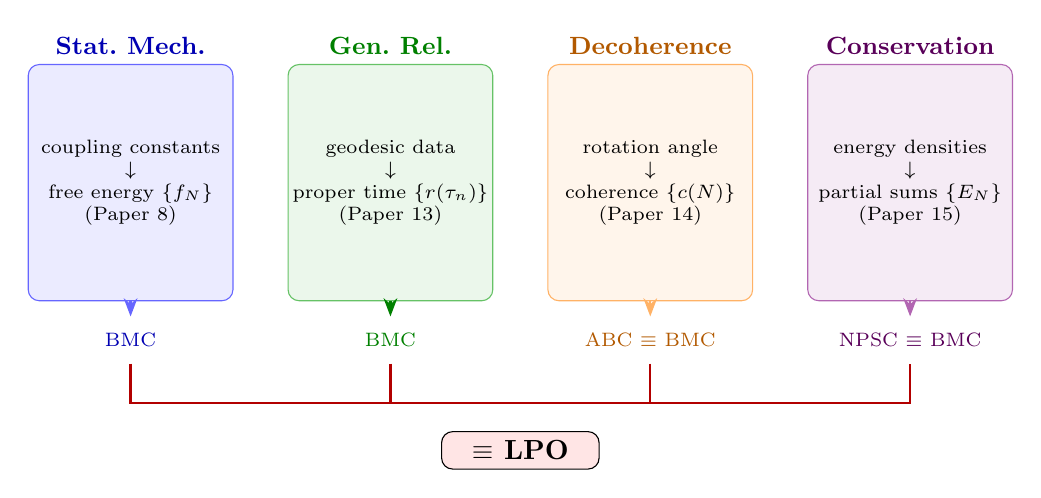
\begin{tikzpicture}[
  pillar/.style={draw, rounded corners, minimum width=2.6cm, minimum height=3cm,
    fill=#1!8, draw=#1!60},
  plabel/.style={font=\small\bfseries, #1},
  >=Stealth
]
% Four pillars
\node[pillar=blue] (sm) at (0,0) {};
\node[plabel=blue!70!black, above] at (sm.north) {Stat.\ Mech.};
\node[font=\scriptsize, align=center] at (sm.center) {coupling constants\\$\downarrow$\\free energy $\{f_N\}$\\(Paper~8)};

\node[pillar=green!60!black] (gr) at (3.3,0) {};
\node[plabel=green!50!black, above] at (gr.north) {Gen.\ Rel.};
\node[font=\scriptsize, align=center] at (gr.center) {geodesic data\\$\downarrow$\\proper time $\{r(\tau_n)\}$\\(Paper~13)};

\node[pillar=orange] (dc) at (6.6,0) {};
\node[plabel=orange!70!black, above] at (dc.north) {Decoherence};
\node[font=\scriptsize, align=center] at (dc.center) {rotation angle\\$\downarrow$\\coherence $\{c(N)\}$\\(Paper~14)};

\node[pillar=violet] (cl) at (9.9,0) {};
\node[plabel=violet!70!black, above] at (cl.north) {Conservation};
\node[font=\scriptsize, align=center] at (cl.center) {energy densities\\$\downarrow$\\partial sums $\{E_N\}$\\(Paper~15)};

% Convergence labels below pillars
\node[font=\scriptsize, blue!70!black] at (0,-2) {BMC};
\node[font=\scriptsize, green!50!black] at (3.3,-2) {BMC};
\node[font=\scriptsize, orange!70!black] at (6.6,-2) {ABC $\equiv$ BMC};
\node[font=\scriptsize, violet!70!black] at (9.9,-2) {NPSC $\equiv$ BMC};

% Arrows down from pillars
\draw[->, thick, blue!60] (sm.south) -- (0,-1.7);
\draw[->, thick, green!50!black] (gr.south) -- (3.3,-1.7);
\draw[->, thick, orange!60] (dc.south) -- (6.6,-1.7);
\draw[->, thick, violet!60] (cl.south) -- (9.9,-1.7);

% Connecting arch to LPO
\draw[thick, red!70!black] (0,-2.3) -- (0,-2.8) -- (9.9,-2.8) -- (9.9,-2.3);
\draw[thick, red!70!black] (3.3,-2.3) -- (3.3,-2.8);
\draw[thick, red!70!black] (6.6,-2.3) -- (6.6,-2.8);
\node[draw, rounded corners, fill=red!10, font=\bfseries, minimum width=2cm] at (4.95,-3.4) {$\equiv$ LPO};

\end{tikzpicture}%
}% end resizebox
\caption{Domain invariance of the BMC~$\equiv$~LPO calibration.
Four independent physical domains each produce a bounded monotone sequence
whose completed-limit existence costs exactly LPO\@.
The surface mechanism varies---direct convergence in statistical mechanics
\cite{Lee2026c} and general relativity \cite{Lee2026paper13},
sign-flip (ABC) in decoherence \cite{Lee2026j},
and telescoping (NPSC) in conservation laws \cite{Lee2026k}---but
the underlying logical structure is invariant.}
\label{fig:domain-invariance}
\end{figure}

\begin{keymessage}
\textbf{Hypothesis:} empirical predictions are BISH-derivable; stronger logic enters only through idealizations no finite laboratory can instantiate.
This is not operationalism---it distinguishes physical content (BISH) from mathematical infrastructure (WLPO/LPO/LEM).
The non-constructive superstructure is not wrong; it is \emph{physically idle}.
\end{keymessage}

% ============================================================
\section{Objections and Open Problems}
% ============================================================

Intellectual honesty requires confronting the strongest objections.

\emph{``The constructive hierarchy tracks mathematical generality, not physical depth.''}
If the correlation between logical strength and idealization were merely a reflection of mathematical complexity---simple theorems are constructive, deep theorems are not---the hypothesis would be trivial.
But the correlation is between logical strength and \emph{physical accessibility}: whether a finite laboratory can instantiate the objects described.
The error bounds for the Ising model are mathematically non-trivial---they involve transfer matrix eigenvalues, logarithmic estimates, and geometric series analysis---but they are BISH because every object in the proof is finitely constructible.
The thermodynamic limit is mathematically elementary---it is just a limit of a monotone sequence---but it requires LPO because the limiting object is infinitely far from any finite approximation in a precise logical sense.
The hierarchy tracks physical accessibility, not mathematical sophistication.

\emph{``What about essential idealizations?''}
Batterman \cite{Batterman2005} has argued that infinite idealizations are ``explanatorily essential''---that the thermodynamic limit, for instance, is not merely a convenience but genuinely explains universality and critical phenomena in a way that finite-system descriptions do not.
We now take a position.
The idealizations are \emph{cognitively} essential: they convert BISH processes into mathematical objects that can be composed, differentiated, and reasoned about at a level of abstraction that finite descriptions cannot match at comparable cognitive cost (Section~\ref{sec:alternatives}).
But they are not \emph{computationally} essential: every number the explanation generates is extractable at BISH\@.
The calibration table measures the logical cost of this cognitive infrastructure.
The cost is real; the benefit is real; the computational content is zero.

\emph{``Doesn't Dyson's divergence of the perturbation series undermine the claim that QED predictions are BISH?''}
No---the opposite.
The finite-order truncation \emph{is} the BISH content.
The divergence of the full series is an LPO-level statement about the cathedral: it asserts that a particular infinite object (the formal sum of all loop orders) fails to converge.
But the predictions come from the truncation, not the sum.
The fact that truncated perturbation theory produces the most precise predictions in physics is precisely the cellar-and-cathedral pattern: the cellar (finite-order Feynman diagrams) delivers the predictions; the cathedral (the infinite series, the path integral, the non-perturbative completion) organizes them.
Dyson's result shows that the cathedral is asymptotic, not convergent---which, if anything, strengthens the case that the physics lives in the cellar.
The justification for trusting the truncation---that the first $n$ terms of an asymptotic series approximate the true value with error bounded by the $(n{+}1)$th term---is itself a BISH-level finite error estimate, even though the asymptotic analysis that establishes this bound may invoke classical techniques.
In effective field theory, the truncation order is set by the energy scale and desired precision---a constructive criterion---not by convergence of the infinite series.

\emph{``Is formulation-invariance robust?''}
The formulation-invariance test---identical axiom profiles across two independent derivations \cite{Lee2026e}---is evidence, not proof.
Two formulations yielding the same logical cost is more compelling than one, but a definitive ineliminability theorem---proving that \emph{any} constructive proof of Ising free energy convergence must use LPO---remains open.

\emph{Open problems.}
Several questions remain genuinely unresolved.
Is there a physical statement whose logical cost is exactly LLPO (the Lesser Limited Principle of Omniscience, strictly weaker than WLPO in the omniscience hierarchy)?
The constructive hierarchy jumps from singular states (WLPO) to the thermodynamic limit (LPO) without stopping at this level.
Does nature skip this step, or have we not found the right example?
What is the constructive cost of renormalization group flows in quantum field theory?
Can the GNS construction---the passage from abstract $C^*$-algebraic states to Hilbert space representations---be calibrated?
How does the D\"oring-Isham topos programme \cite{DoeringIsham2008}, which arrives at intuitionistic logic through a completely different route, relate to the constructive hierarchy?

And the deepest open problem of all: what is \emph{the principle}?
The calibration table establishes a correlation between logical strength and physical idealization.
A fully satisfying account would provide a single physical principle---analogous to the constancy of the speed of light or the equivalence principle---from which the correlation \emph{follows}.
Why BISH?
What is it about the physical world that makes constructive logic the right logic for empirical predictions?
No one has this principle.
Finding it would transform the correlation into a theorem and the hypothesis into a physical law.
Such a principle would be a physical postulate---analogous to ``no superluminal signaling'' or ``the equivalence of inertial frames''---from which BISH-derivability of empirical content follows as a consequence.
The calibration table constrains what such a principle can say; it does not yet say it.
It remains the most important open problem the research programme has generated.
Whether the persistent appearance of BISH-level empirical content across both gravitational and quantum theories constrains the space of viable quantum gravity programmes---by requiring that their predictions, too, be extractable without omniscience principles---is a question the calibration table motivates but does not answer.

\begin{keymessage}
The hierarchy tracks physical accessibility, not mathematical sophistication.
The correlation between logical strength and idealization is robust but not yet explained by a single principle.
The deepest open problem: what physical principle explains why nature speaks the language of constructive logic?
\end{keymessage}

% ============================================================
\section{Return to the Cellar}
% ============================================================

Return to the anomalous magnetic moment of the electron.

The number that theory and experiment agree on, to twelve decimal places, is a BISH computation.
Finite Feynman diagrams, finite integrals, finite arithmetic.
The cathedral of infinite-dimensional mathematical physics sits above this number: beautiful, useful as a thinking device, and largely idle as far as predictions are concerned.

The constructive hierarchy---developed by Brouwer for philosophical reasons, refined by Bishop \cite{Bishop1967} for mathematical reasons, and sharpened by Bridges, Ishihara \cite{Ishihara1992, Ishihara2006}, and their students into a precise instrument of logical calibration---turns out to be the right tool for mapping the boundary between the physical world and the mathematical structures we use to describe it.
It was not designed for this purpose.
That it answers questions about the foundations of physics is either a coincidence or evidence that the questions are the same question.

Whether nature is constructive is a hypothesis, not a theorem.
The evidence is machine-verified: approximately 12,000~lines of Lean~4 proofs with auditable axiom certificates across quantum mechanics, statistical mechanics, general relativity, open quantum systems, and conservation laws.
The hypothesis could be wrong---a single empirical prediction that provably requires LPO would refute it.
It is stated precisely enough to be falsifiable, which is all one can ask of a scientific proposal.

We now have the tool.
The calibration table tells us where the map matches the territory and where the mapmaker's conventions begin.
What remains is finding the principle that explains why the physical world speaks the language of constructive logic, if indeed it does.

The most precise prediction in physics requires the least logical strength.
That may be the most important thing the prediction tells us.

% ============================================================
\begin{thebibliography}{99}

\bibitem{Batterman2005}
R.~W.~Batterman,
``Critical phenomena and breaking drops: infinite idealizations in physics,''
\emph{Studies in History and Philosophy of Modern Physics} \textbf{36} (2005), 225--244.

\bibitem{Bishop1967}
E.~Bishop,
\emph{Foundations of Constructive Analysis},
McGraw-Hill, New York, 1967.

\bibitem{BridgesRichman1987}
D.~Bridges and F.~Richman,
\emph{Varieties of Constructive Mathematics},
Cambridge University Press, 1987.

\bibitem{BridgesVita2006}
D.~Bridges and L.~S.~V\^{\i}\c{t}\u{a},
\emph{Techniques of Constructive Analysis},
Springer, New York, 2006.

\bibitem{Cubitt2015}
T.~S.~Cubitt, D.~Perez-Garcia, and M.~M.~Wolf,
``Undecidability of the spectral gap,''
\emph{Nature} \textbf{528} (2015), 207--211.

\bibitem{DoeringIsham2008}
A.~D\"oring and C.~J.~Isham,
``\,`What is a thing?': Topos theory in the foundations of physics,''
in \emph{New Structures for Physics}, Lecture Notes in Physics \textbf{813}, Springer, 2008.

\bibitem{Dyson1952}
F.~J.~Dyson,
``Divergence of perturbation theory in quantum electrodynamics,''
\emph{Physical Review} \textbf{85}(4) (1952), 631--632.

\bibitem{Einstein1939}
A.~Einstein,
``On a stationary system with spherical symmetry consisting of many gravitating masses,''
\emph{Annals of Mathematics} \textbf{40} (1939), 922--936.

\bibitem{JNVWY2021}
Z.~Ji, A.~Natarajan, T.~Vidick, J.~Wright, and H.~Yuen,
``{MIP}$^*$ = {RE},''
\emph{Communications of the ACM} \textbf{64}(11) (2021), 131--138.

\bibitem{Gisin2020}
N.~Gisin,
``Mathematical languages shape our understanding of time in physics,''
\emph{Nature Physics} \textbf{16} (2020), 114--116.

\bibitem{Gisin2021}
N.~Gisin,
``Indeterminism in physics, classical chaos and Bohmian mechanics: Are real numbers really real?''
\emph{Erkenntnis} \textbf{86} (2021), 1469--1481.

\bibitem{GlimmJaffe1981}
J.~Glimm and A.~Jaffe,
\emph{Quantum Physics: A Functional Integral Point of View},
Springer, New York, 1981.

\bibitem{Haag1996}
R.~Haag,
\emph{Local Quantum Physics: Fields, Particles, Algebras},
2nd ed., Springer, Berlin, 1996.

\bibitem{Ishihara1992}
H.~Ishihara,
``Continuity properties in constructive mathematics,''
\emph{Journal of Symbolic Logic} \textbf{57} (1992), 557--565.

\bibitem{Ishihara2006}
H.~Ishihara,
``Reverse mathematics in Bishop's constructive mathematics,''
\emph{Philosophia Scientiae}, Cahier sp\'ecial \textbf{6} (2006), 43--59.

\bibitem{Kerr2023}
R.~P.~Kerr,
``Do black holes have singularities?''
Preprint, arXiv:2312.00841, 2023.

\bibitem{Lee2026a}
P.~C.-K.~Lee,
``Constructive reverse mathematics of the bidual gap: WLPO equivalence for Banach space non-reflexivity,''
2026. Zenodo DOI: 10.5281/zenodo.17107493.

\bibitem{Lee2026b}
P.~C.-K.~Lee,
``The physical bidual gap: WLPO and non-reflexivity of trace-class operators,''
2026. Zenodo DOI: 10.5281/zenodo.18509795.

\bibitem{Lee2026c}
P.~C.-K.~Lee,
``The constructive cost of the thermodynamic limit: LPO equivalence and BISH dispensability in the 1D Ising model,''
2026. Zenodo DOI: 10.5281/zenodo.18516813.

\bibitem{Lee2026e}
P.~C.-K.~Lee,
``Formulation-invariance of the logical cost of the thermodynamic limit: a combinatorial proof for the 1D Ising model,''
2026. Zenodo DOI: 10.5281/zenodo.18517570.

\bibitem{Lee2026f}
P.~C.-K.~Lee,
``Axiom calibration for quantum spectra: orthogonal heights, choice principles, and separation portals,''
2026. Zenodo DOI: 10.5281/zenodo.17059483.

\bibitem{Lee2026g}
P.~C.-K.~Lee,
``Constructive reverse mathematics for the Heisenberg uncertainty principle: Robertson-Schr\"odinger and Schr\"odinger inequalities over Mathlib,''
2026. Zenodo DOI: 10.5281/zenodo.18519836.

\bibitem{Lee2026paper10}
P.~C.-K.~Lee,
``The logical geography of mathematical physics: constructive calibration from density matrices to the event horizon,''
2026. Zenodo DOI: 10.5281/zenodo.18527559.

\bibitem{Lee2026paper11}
P.~C.-K.~Lee,
``Constructive entanglement: CHSH, Tsirelson bound, and Bell state entropy at BISH,''
2026. Zenodo DOI: 10.5281/zenodo.18527676.

\bibitem{Lee2026paper13}
P.~C.-K.~Lee,
``The event horizon as a logical boundary: Schwarzschild interior geodesic incompleteness and LPO in Lean~4,''
2026. Preprint. Paper~13 in the CRM series.

\bibitem{Lee2026j}
P.~C.-K.~Lee,
``Constructive decoherence: exact environment limits, LPO equivalence, and BISH bounds for open quantum systems,''
2026. Paper~14 in the CRM series.

\bibitem{Lee2026k}
P.~C.-K.~Lee,
``Constructive Noether: local conservation at BISH, global energy at LPO,''
2026. Paper~15 in the CRM series.

\bibitem{Lee2026l}
P.~C.-K.~Lee,
``The Born rule at BISH: finite-dimensional measurement probabilities and frequentist convergence at DC$_\omega$,''
2026. Paper~16 in the CRM series.

\bibitem{OppenheimerSnyder1939}
J.~R.~Oppenheimer and H.~Snyder,
``On continued gravitational contraction,''
\emph{Physical Review} \textbf{56} (1939), 455--459.

\bibitem{Penrose1965}
R.~Penrose,
``Gravitational collapse and space-time singularities,''
\emph{Physical Review Letters} \textbf{14}(3) (1965), 57--59.

\bibitem{Raychaudhuri1955}
A.~K.~Raychaudhuri,
``Relativistic cosmology.~I,''
\emph{Physical Review} \textbf{98} (1955), 1123--1126.

\bibitem{Redei1996}
M.~R\'edei,
``Why John von Neumann did not like the Hilbert space formalism of quantum mechanics (and what he liked instead),''
\emph{Studies in History and Philosophy of Modern Physics} \textbf{27}(4) (1996), 493--510.

\bibitem{vanDalen2005}
D.~van~Dalen,
\emph{Mystic, Geometer, and Intuitionist: The Life of L.~E.~J.~Brouwer}, Vol.~2,
Clarendon Press, Oxford, 2005.

\bibitem{vanWierst2019}
P.~van~Wierst,
``The paradox of phase transitions in the light of constructive mathematics,''
\emph{Synthese} \textbf{196} (2019), 1863--1884.

\bibitem{vonNeumann1932}
J.~von~Neumann,
\emph{Mathematische Grundlagen der Quantenmechanik},
Springer, Berlin, 1932.

\bibitem{Weyl1918}
H.~Weyl,
\emph{Das Kontinuum: Kritische Untersuchungen \"uber die Grundlagen der Analysis},
Veit, Leipzig, 1918.

\bibitem{Wilson1974}
K.~G.~Wilson,
``Confinement of quarks,''
\emph{Physical Review D} \textbf{10}(8) (1974), 2445--2459.

\bibitem{BoussoPolchinski2000}
R.~Bousso and J.~Polchinski,
``The string theory landscape,''
\emph{Journal of High Energy Physics} \textbf{2000}(06) (2000), 006.

\bibitem{Susskind2003}
L.~Susskind,
``The anthropic landscape of string theory,''
in \emph{Universe or Multiverse?}, ed.\ B.~Carr, Cambridge University Press, 2003.
arXiv:hep-th/0302219.

\bibitem{AMPS2013}
A.~Almheiri, D.~Marolf, J.~Polchinski, and J.~Sully,
``Black holes: complementarity vs.\ firewalls,''
\emph{Journal of High Energy Physics} \textbf{2013}(02) (2013), 062.

\end{thebibliography}

\bigskip
\section*{Statement of AI Use}

This essay was written with the assistance of Anthropic's Claude Opus~4.6.
The author's primary training is in interventional cardiology, not mathematical logic or mathematical physics; his main research interests are in applicational AI and medicine.
The formal results described herein are machine-verified in Lean~4, which is precisely the tool that decouples the validity of the proofs from the credentials of the prover.
The expository narrative should be read with this context in mind.

\bigskip
\noindent\textit{For Mimi, my wife, who always knew the cellar was enough.}

\end{document}
